%%%%%%%%%%%%%%%%%%%%%%%%%%%%%%%%%%%%%%%%%%%%%%%%%%%%%%%%%%%%
%%% ELIFE ARTICLE TEMPLATE
%%%%%%%%%%%%%%%%%%%%%%%%%%%%%%%%%%%%%%%%%%%%%%%%%%%%%%%%%%%%
%%% PREAMBLE 
\documentclass[9pt,lineno]{elife}
% Use the onehalfspacing option for 1.5 line spacing
% Use the doublespacing option for 2.0 line spacing
% Please note that these options may affect formatting.
% Additionally, the use of the \newcommand function should be limited.


\usepackage{lipsum} % Required to insert dummy text
\usepackage[version=4]{mhchem}
\usepackage{siunitx}
\usepackage[export]{adjustbox}
\usepackage{float}
\DeclareSIUnit\Molar{M}

\newcommand{\jdbcomment}[1]{\emph{\color{red} [#1]}}
\newcommand{\abrcomment}[1]{\emph{\color{blue} [#1]}}

\renewcommand{\floatpagefraction}{.9}

\newfloat{suppfile}{thp}{lofsupfile}
%\renewcommand{\thesuppfile}{Supplementary file \arabic{suppfile}}
\floatname{suppfile}{Supplementary file}

%%%%%%%%%%%%%%%%%%%%%%%%%%%%%%%%%%%%%%%%%%%%%%%%%%%%%%%%%%%%
%%% ARTICLE SETUP
%%%%%%%%%%%%%%%%%%%%%%%%%%%%%%%%%%%%%%%%%%%%%%%%%%%%%%%%%%%%
\title{Single-cell virus sequencing of influenza infections that trigger innate immunity}

\author[1]{Alistair B. Russell}
\author[1]{Jacob R. Kowalsky}
\author[1,2,3*]{Jesse D. Bloom}
\affil[1]{Basic Sciences Division and Computational Biology Program, Fred Hutchinson Cancer Research Center, Seattle, United States}
\affil[2]{Department of Genome Sciences, University of Washington, Seattle, United States}
\affil[3]{Howard Hughes Medical Institute, Fred Hutchinson Cancer Research Center, Seattle, United States}

\corr{jbloom@fredhutch.org}{JDB}

%%%%%%%%%%%%%%%%%%%%%%%%%%%%%%%%%%%%%%%%%%%%%%%%%%%%%%%%%%%%
%%% ARTICLE START
%%%%%%%%%%%%%%%%%%%%%%%%%%%%%%%%%%%%%%%%%%%%%%%%%%%%%%%%%%%%

\begin{document}

\maketitle

\begin{abstract}
The outcome of viral infection is extremely heterogeneous at the level of individual cells, including sparse activation of innate immunity.  
Here we assess how the genetic variation inherent in viral populations contributes to this heterogeneity.
We do this by developing a new approach to determine both the transcriptome and full-length sequences of all viral genes in single influenza-infected cells.
Infections that activate an innate-immune response in single cells are associated with viral defects that include amino-acid mutations, internal deletions, and failure to express key genes.  
However, immune activation remains stochastic in cells infected by virions with these defects, and sometimes occurs even in cells infected by virions that express unmutated copies of all genes.
Our work shows that the genetic variation present in influenza virus populations substantially contributes to but does not fully explain the heterogeneity in infection outcome and immune activation in single infected cells.
\end{abstract}


\section{Introduction}
Infection with an acute virus such as influenza initiates a race between the virus and immune system.
As the virus spreads, some infected cells trigger innate immunity and begin producing interferon (IFN).
This IFN directs expression of anti-viral interferon-stimulated genes (ISGs) in the infected cell and its neighbors via autocrine and paracrine signaling, as well as helping launch a broader immune response~\citep{stetson2006type,honda2006type}.
If innate immunity is activated sufficiently rapidly, it can reduce viral replication and disease severity~\citep{solov1969results,treanor1987intranasally,beilharz2007protection,kugel2009intranasal,steel2010transmission}---although excessive immune responses later in infection can actually be associated with immunopathology and more severe disease~\citep{la2007question, iwasaki2014innate}.

Unfortunately for the host, influenza infection only rarely triggers IFN production by individual infected cells early in infection~\citep{kallfass2013visualizing, killip2017single}.
This rareness of IFN induction is just one form of the extreme cell-to-cell heterogeneity that characterizes influenza infection: infected cells also vary widely in their production of viral mRNA, proteins, and progeny virions~\citep{russell2018extreme,steuerman2018dissection,sjaastad2018distinct,heldt2015single}.
Because viral replication and the IFN response are both feed-forward processes, early cell-to-cell heterogeneity could have significant downstream consequences for the race between virus and immune system---especially as real influenza infections are typically initiated by just a few virions entering a few cells~\citep{mccrone2018stochastic, xue2018reconciling, varble2014influenza}.

It is unclear why only some infected cells trigger innate-immune responses.
Two possible contributors are pure stochasticity and pre-existing variation in cellular state.
For instance, only some cells induce IFN even upon homogeneous treatment with synthetic innate-immune ligands~\citep{shalek2013single, shalek2014single, wimmers2018single}, and the frequency of IFN induction may depend on a cell's pre-existing chromatin state~\citep{bhushal2017cell}.
But for influenza, a third possible contributor also looms large: viral genetic diversity.
Because influenza has a high mutation rate, even if the \emph{consensus} sequence of a viral population is ``wild-type,'' individual virions will often have defects~\citep{parvin1986measurement, suarez1992heterogeneity, suarez1994estimation, bloom2014experimentally, pauly2017novel}.
Indeed, many studies have identified mutations that increase IFN induction when engineered into a viral population~\citep{velthuis2018mini, du2018genome, killip2017single, perez2014unbiased}, and viral stocks that are rich in internal deletions in the polymerase genes induce more IFN~\citep{baum2010preference, tapia2013defective, boergeling2015evidence, dimmock2015cloned}.

However, existing techniques are inadequate to determine how viral genetic diversity contributes to cell-to-cell heterogeneity during infection, since they do not determine full sequences of the virions that infect individual cells.
Flow cytometry and fluorescent reporters only measure protein levels~\citep{brooke2013most, guo2017single}, and current single-cell transcriptomic techniques primarily measure abundance of transcripts and provide only fragmentary information on their sequences~\citep{russell2018extreme, zanini2018single, zanini2018virus, steuerman2018dissection, saikia2018simultaneous}.
None of these techniques reliably reveal if the virion infecting a specific cell has some idiosyncratic mutation, despite the fact that such mutations are common regardless of whether the cells are infected with a nominally ``wild-type'' or ``mutant'' stock of virus.

Here we develop a new approach to measure both the full transcriptome and the sequences of all viral genes in single influenza-infected cells.
To do this, we first enrich for rare IFN+ cells, and then perform both standard Illumina-based single-cell transcriptomics and full-length PacBio sequencing of viral genes.
We obtain the transcriptomes and full sequences of all expressed viral genes in 150 infected cells, 40 of which express IFN.
Even though we used a nominally ``wild-type'' stock of virus, two-thirds of cells are infected by virions that have a mutation or defect in gene expression.
This viral diversity is a major contributor to cell-to-cell heterogeneity, with cells infected by truly wild-type virions having a tighter distribution of viral transcriptional burden.
Viral defects are especially common in IFN+ cells, and we identify at least four defects that cause increased IFN induction: amino-acid substitutions in the viral polymerase (PB1), absence of the NS gene, amino-acid substitutions in NS1, and internal deletions in polymerase genes.
However, viral genetic variation does not fully explain the cell-to-cell heterogeneity, as even truly wild-type virions sometimes induce IFN, and no viral mutations deterministically induce IFN.
Therefore, viral diversity is an important but not exclusive cause of cell-to-cell heterogeneity during influenza infection.

\section{Results}

\subsection{A system to identify and enrich for rare IFN+ positive cells}
A challenge in studying IFN induction by influenza virus is that infection only rarely triggers expression of anti-viral IFN~\citep[type I and type III;][]{kotenko2017contribution} at the level of single-cells ~\citep{killip2017single}.
For instance, we previously performed single-cell transcriptomics on hundreds of influenza-infected A549 human lung epithelial cells at early times (6 to 10 hours) post-infection~\citep{russell2018extreme}.
Only 1 of 368 infected cells expressed detectable type I or type III IFN (\FIG{IFNrare}A).
This paucity of IFN+ cells was not due simply to a poor detection threshold, since $>$100 IFN transcripts were detected in the one IFN+ cell~\citep{russell2018extreme}.

This rareness of IFN induction is not merely a feature of A549 cells in culture.
Prior studies using interferon reporter constructs have found that IFN expression is rare in influenza-infected mice at 24 and even 48 hours post-infection~\citep{kallfass2013visualizing}.
In support of these findings, we re-analyzed the single-cell transcriptomics of influenza-infected mice by \citet{steuerman2018dissection}.
As shown in \FIGSUPP[IFNrare]{mice}, many infected cells in the mice expressed IFN-stimulated genes (ISGs), which are induced by autocrine and paracrine signaling~\citep{stetson2006type,honda2006type}.
But just a handful of cells detectably expressed IFN itself, which is only induced by direct cellular detection of viral infection~\citep{stetson2006type,honda2006type}.

%%% start IFNrare figure %%%
\begin{figure}
\centerline{
{\bf \Large A}\includegraphics[width=0.25\textwidth,valign=t]{figures/IFN_stochastic/RussellVenn/venn_diagram.pdf}
\hspace{0.02\textwidth}
{\bf \Large B}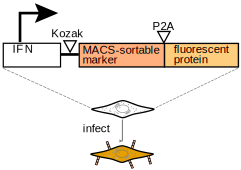
\includegraphics[width=0.32\textwidth,valign=t]{figures/IFN_stochastic/IFN_reporter/IFN_reporter.pdf}
\hspace{0.02\textwidth}
{\bf \Large C} \includegraphics[width=0.2\textwidth,valign=t]{figures/IFN_stochastic/Flow/ifn_percent.pdf}
}
\caption{
IFN expression is rare in influenza-infected cells.
{\bf (A)} Number of infected and IFN+ A549 cells in our prior single-cell transcriptomics~\citep{russell2018extreme}.
\FIGSUPP[IFNrare]{mice} shows that IFN+ cells were also rare in the single-cell transcriptomics of influenza-infected mice by \citet{steuerman2018dissection}.
{\bf (B)} An A549 reporter cell line to identify cells expressing IFN.
The reporter consists of an IFN promoter that drives expression of a cell-surface protein amenable to MACS and a fluorescent protein.
We created reporters with type I and type III IFN promoters (\FIGDATA[IFNrare]{reporter_sequences}).
The reporters were efficiently activated by an IFN-inducing strain of Sendai virus (\FIGSUPP[IFNrare]{reporter_validation}).
{\bf (C)}
Frequency of IFN induction upon infection with the influenza virus stock used in the single-cell studies in this paper, as quantified using the reporter cell line (see \FIGSUPP[IFNrare]{flow} for details).
The plot also shows uninfected cells, and cells infected with saturating amounts of Sendai virus.
The limit of detection of 0.05\% is indicated with a dashed line, and numbers show the median of three measurements.
}
\label{fig:IFNrare}

\figsupp[Few cells express detectable IFN in influenza-infected mice.]
{A re-analysis of the data from \citet{steuerman2018dissection}'s single-cell transcriptomics of cells from influenza-infected mice shows that only 5 of 1220 virus-infected cells express \emph{detectable} type I or type III IFN transcripts \textit{in vivo}.
Specifically, we downloaded the data from \citet{steuerman2018dissection} and identified influenza-infected cells using criteria similar to those described in \citet{steuerman2018dissection}.
Here we show statistics for the cells from the influenza-infected wild-type C57BL/6J mice, which were collected at 48 hours (two replicates) or 72 hours (one replicate)---we do not show cells from the control mice.
As shown in the left-most panel, the sequencing depth of \citet{steuerman2018dissection} was quite low, with only $\sim$1,500 mRNA counts per cell on average (this is 10 to 15-fold lower than the sequencing depth in \citet{russell2018extreme} and the current study, respectively).
An important caveat is that this low sequencing depth could lead to a simple failure to detect IFN transcripts in some cells.
Nonetheless, there is detectable expression of key ISGs in the majority of infected cells (the middle panel shows the total counts of IFIT1, ISG15, CCL5, and Mx1).
However, only 5 of 1220 cells express any detectable type I (IFN-$\alpha$ and IFN-$\beta$) or type III (IFN-$\lambda$) mRNAs, and only at low levels (one transcript detected).
The full code that performs the re-analysis shown in this figure is at \url{https://github.com/jbloomlab/IFNsorted_flu_single_cell/tree/master/paper/figures/IFN_stochastic/SteuermanReanalysis/}.
}
{\includegraphics[width=\textwidth]{figures/IFN_stochastic/SteuermanReanalysis/plots/p_mRNA_counts.pdf}}
\label{figsupp:mice}

\figsupp[Validation of IFN reporter cell lines.]
{To validate the IFN reporter cell lines, they were infected at high MOI with the Cantell strain of Sendai virus, which strongly activates IFN expression~\citep{strahle2006sendai}.
The name of each of reporter cell line is indicated at the top of each row of plots.
At 13 hours post-infection, activation of the IFN reporter was then monitored by flow cytometry using the marker indicated at the bottom of each plot (either a fluorescent protein or antibody staining for the cell-surface LNGFR$\Delta$C using a PE-conjugated anti-LNGFR antibody from Miltenyi Biotec).
Sendai infection efficiently activated the IFN reporter in all cases, with the strongest signal from the IFN-$\lambda$ reporter driving ZsGreen.
}
{\includegraphics[width=0.5\textwidth]{figures/IFN_stochastic/IFN_reporter/Sendai_validation.pdf}}
\label{figsupp:reporter_validation}

\figsupp[Expression of type I and type III IFN is highly correlated in A549 cells.]
{An A549 cell line was generated by transduction with both the IFN-$\beta$ and IFN-$\lambda$ reporters driving expression of mCherry and ZsGreen, respectively.
The cells were then infected with two different stocks of ``wild-type'' WSN influenza, or stocks with a deletion in PB1 or stop codons in NS1 (described later in the paper).
After 13 hours, cells were analyzed by flow cytometry.
As shown in the FACS plots, expression of the \textit{IFNB1} and \textit{IFNL1} reporters is highly correlated in all cases.}
{\includegraphics[width=0.5\textwidth]{figures/IFN_stochastic/IFN_reporter/IFNbeta_IFN_lambda_correlated.pdf}}
\label{figsupp:type_I_vs_III}

\figsupp[Full flow cytometry data for \FIG{IFNrare}C.]
{Flow cytometry data for \FIG{IFNrare}C.
The A549 cells with the \textit{IFNL1} reporter driving LNGFR$\Delta$C-ZsGreen were not infected, infected with saturating amounts of the Cantell strain of Sendai virus~\citep{strahle2006sendai}, or infected the same stock of influenza virus used in the single-cell experiment at a target MOI of 0.3.
After 13 hours, the cells were stained for expression of HA protein and analyzed by FACS for HA and expression of the ZsGreen driven by the \textit{IFNL1} reporter.
Each condition was done in triplicate.
The contour plots show the density of all cells, and all IFN+ cells are also indicated by orange dots.
Cells were classified as HA+ or IFN+ based on gates set to put 0.05\% of the uninfected cells in these populations.
For the influenza-infected cells, the percentage IFN+ was calculated only among the HA+ cells (since these are the ones that are infected).
For the uninfected and Sendai-virus infected, the percentage IFN+ was calculated among all cells, since these cells do not express HA.
}
{\includegraphics[width=0.75\textwidth]{figures/IFN_stochastic/Flow/flow_plot.pdf}}
\label{figsupp:flow}

\figdata{Sequences of the reporters in \FIG{IFNrare}B are at \url{https://github.com/jbloomlab/IFNsorted_flu_single_cell/tree/master/paper/figures/IFN_stochastic/IFN_reporter/1517_pHAGE2_IFNbeta_prom_LNGFR_P2A_mNeongreen.gb} and \url{https://github.com/jbloomlab/IFNsorted_flu_single_cell/tree/master/paper/figures/IFN_stochastic/IFN_reporter/1767_pHAGE2_IL29_promnkozak_LNGFR_P2A_zsGreen.gb}.
}
\label{figdata:reporter_sequences}

\end{figure}
%%% end IFNrare figure %%%

To efficiently identify and enrich rare IFN+ cells, we integrated IFN reporters into the genome of A549 cells (\FIG{IFNrare}B) using lentiviral transduction and subsequently propagated these reporters from single clones.
These reporters consisted of a type I (\textit{IFNB1}) or type III (\textit{IFNL1}) promoter driving expression of a cell-surface protein~\citep[LNGFR$\Delta$C;][]{bonini1997hsv,ruggieri1997cell} followed by a fluorescent protein.
Cells that activate the IFN reporter can enriched by magnetic-activated cell sorting (MACS) for the cell-surface protein, or identified by flow cytometry for the fluorescent protein.
The reporters were efficiently activated by a strain of Sendai virus~\citep{strahle2006sendai} that potently induces IFN (\FIGSUPP[IFNrare]{reporter_validation}), and activation of the type I and type III IFN reporters was highly correlated in single influenza-infected A549 cells (\FIGSUPP[IFNrare]{type_I_vs_III}; further validated by the single-cell transcriptomics described below).
Therefore, for the rest of this paper, we use ``IFN expression'' to refer to combined expression of type I and III IFNs. 

We used the reporter cells to quantify the frequency of IFN induction in A549 cells infected with the A/WSN/1933 (H1N1) strain of influenza (hereafter referred to as ``WSN'').
As shown in \FIG{IFNrare}C, $\sim$0.5\% of infected cells activated the IFN reporter at 13 hours post-infection.
This frequency of IFN induction is roughly comparable to that observed in our prior single-cell transcriptomics of influenza-infected cells (\FIG{IFNrare}B).

\subsection{Combined transcriptomics and virus-sequencing of single infected cells}
We next developed a method to determine if features of the infecting virions are responsible for the heterogeneous outcome of infection in single cells.
Standard single-cell transcriptomic techniques are inadequate for this purpose, since they just use 3'-end sequencing of poly-adenylated mRNAs to measure the abundance of each transcript~\citep{klein2015droplet, macosko2015highly, zheng2017massively, cao2017comprehensive, gierahn2017seq}, and do not reveal if the virions that infect individual cells have features (e.g., mutations) that contribute to heterogeneity in infection outcome. 

%%% start workflow figure
\begin{figure}
\begin{fullwidth}

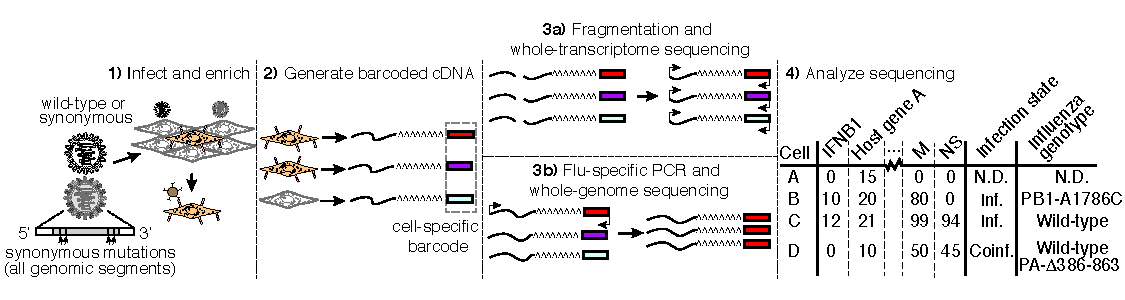
\includegraphics[width=\linewidth, valign=t]{figures/WorkflowSchematic/SchematicForPaper.pdf}

\caption{
Approach for combined transcriptomic and viral sequencing of single influenza-infected cells that express IFN.
{\bf (A)}
IFN reporter A549 cells are infected with a mix of wild-type and synonymously barcoded viruses.
IFN+ cells are enriched by MACS (\FIGSUPP[workflow]{MACS}), and pooled with non-enriched cells and uninfected canine cells that serve as an internal control for multiplets and mRNA leakage.
{\bf (B)}
The mRNAs from individual cells are converted to cDNAs tagged with cell-specific barcodes using the 10X Chromium platform.
{\bf (C)}
Cellular transcriptomes are quantified using standard single-cell 3'-end Illumina sequencing, and 
{\bf (D)}
viral genes are enriched by influenza-specific PCR and fully sequenced by PacBio.
{\bf (E)}wild-type
The result is a matrix giving the expression of each gene in each cell, as well as the full sequences of the viral genes in infected cells.
}
\label{fig:workflow}

\figsupp[MACS enrichment of IFN+ cells.]
{
Example MACS enrichments of IFN+ influenza-infected cells.
A549 cells with the \textit{IFNB1} LNGFR$\Delta$C-mNeonGreen reporter were infected with wild-type WSN influenza (two different viral stocks) at a target MOI of 0.1 TCID50 per cell.
After infection had proceeded for 12 hours, the cells were twice magnetically sorted for LNGFR$\Delta$C expression over magnetic columns as detailed in the methods for the single-cell sequencing experiment.
{\bf (A)}
After sorting, the populations were analyzed by flow cytometry for IFN expression using the mNeonGreen fluorescent protein.
The plots show the distribution of fluorescence in the original population, the flow-through from the first column, and the MACS-sorted positive population after two columns.
As indicated by the percentages shown for the original and MACS-sorted population, this process led to substantial enrichment in IFN+ cells.
We expect that the IFN sorting for the actual single-cell sequencing led to similar enrichment, although we could not directly quantify this as the sorted cells in that case were immediately used for the sequencing and so could not be analyzed by flow cytometry.
{\bf (B)}
Analysis of expression of IFNB1 (relative to the housekeeping gene L32) by qPCR in the positive (IFN enriched) and negative (IFN depleted) populations from panel (A).
The qPCR validates a roughly 50- to 100-fold enrichment in total IFNB1 expression.
The qPCR was performed in quadruplicate (hence the four points for each sample).
}
{\includegraphics[width=\textwidth]{figures/MACS/MACS.pdf}}
\label{figsupp:MACS}

\figdata{Genbank files giving sequences of the wild-type and synonymously barcoded viruses are in \url{https://github.com/jbloomlab/IFNsorted_flu_single_cell/blob/master/data/flu_sequences/flu-wsn.gb} and \url{https://github.com/jbloomlab/IFNsorted_flu_single_cell/blob/master/data/flu_sequences/flu-wsn-double-syn.gb}.}
\label{figdata:virus_seqs}

\end{fullwidth}
\end{figure}
%%% end workflow figure

We therefore developed the approach in \FIG{workflow} to determine the entire transcriptome \emph{and} the full sequences of the infecting virions in single cells.
First, we generated a stock of virus that consisted of a mix of wild-type WSN and a ``synonymously barcoded'' variant that contained two engineered synonymous mutations near each termini of each gene (\FIGDATA[workflow]{virus_seqs}).
These viral barcodes allow us to identify co-infection of individual cells from single-cell transcriptomic data~\citep{russell2018extreme}, and also provide an important control for PCR artifacts during full-length sequencing of viral transcripts (see below).

We next used this viral stock to infect A549 IFN reporter cells (\FIG{workflow}A) at a dose that led to detectable viral transcription in about a quarter of the cells.
From 12 to 13 hours post-infection, we used MACS to enrich cells that had activated the IFN reporter.
Based on pilot experiments, we expected this MACS to enrich IFN+ cells to $\sim$5\% to 30\% of the total (\FIGSUPP[workflow]{MACS}).
To ensure the presence of infected IFN- cells after MACS enrichment, we added back non-enriched cells to $\sim$10\% of the total.
We also added uninfected canine cells to $\sim$5\% of the total as a control for multiplets and to estimate the background amount of viral mRNA detected in truly uninfected cells.

We processed the cells on a commercially available platform~\citep[the 10X Chromium;][]{zheng2017massively} that physically isolates cells in droplets and then reverse transcribes polyadenylated mRNAs to append a unique cell barcode to all cDNAs in each droplet, and a unique molecular identifier (UMI) to each cDNA molecule (\FIG{workflow}B).
Because influenza virus mRNAs are polyadenylated~\citep{robertson1981polyadenylation}, this process appends cell barcodes to both cellular and viral mRNAs.
Furthermore, because virtually the entire influenza genome is transcribed, the cell-barcoded cDNA spans almost all 13,581 nucleotides in the segmented viral genome: the only portions not covered are one universally conserved nucleotide upstream of the transcription start site~\citep{koppstein2015sequencing} and 17 to 22 highly conserved nucleotides downstream of the polyadenylation site~\citep{robertson1981polyadenylation} in each of the eight viral gene segments.

We used a portion of the cell-barcoded cDNA for standard single-cell transcriptomics by Illumina 3'-end sequencing (\FIG{workflow}C).
But we also took a portion and enriched for full-length viral molecules by PCR (\FIG{workflow}D).
We performed PacBio sequencing on these full-length viral cDNAs to generate high-accuracy circular consensus sequences~\citep[CCSs;][]{travers2010flexible}.
These CCSs retain the cell barcodes, and with sufficient sequencing depth we obtain CCSs from multiple unique UMI-tagged cDNAs for each viral gene in each cell.
Because most cells are infected by just one or two virions, we can build a consensus of CCSs for each viral gene in each cell to determine the sequence(s) of these virions.
Combining this information with the 3'-end sequencing determines the entire transcriptome and the full sequences of the infecting virions in single cells (\FIG{workflow}E).

\subsection{Transcriptomic analyses of single IFN+ and IFN- influenza-infected cells}

%%% start transcriptomics figure
\begin{figure}
\begin{fullwidth}

\includegraphics[width=\linewidth, clip=false]{figures/single_cell_figures/p_cell_summary.pdf}

\caption{
Single-cell transcriptomics of IFN-enriched influenza-infected cells.
{\bf (A)} 
Number of cells for which transcriptomes were obtained.
From these numbers, we estimate~\citep{bloom2018estimating} that $\approx$11\% of the transcriptomes are actually multiplets derived from multiple cells. 
{\bf (B)} The number of cellular and viral mRNAs detected for each cell is plotted as a point.
Green lines show the distribution of cellular mRNAs per cell, and the blue rug plot at the left of each panel shows the distribution of viral mRNAs per cell.
Cells outside the dashed magenta lines have unusually low or high amounts of cellular mRNA (likely low-quality emulsions or multiplets), and are excluded from subsequent analyses.
{\bf (C)} Distribution across cells of the fraction of all mRNA derived from influenza.
Cells called as infected are in blue, while other cells are in green.
The inset shows the amount of viral mRNA in the human cells that are called as infected.
{\bf (D)} Number of influenza genes detected per infected cell, and the amount of viral mRNA in cells expressing each number of viral genes.
The majority of cells express all eight gene segments, but a substantial minority fail to express at least one gene.
\FIGSUPP[transcriptomics]{frac_has_gene} shows the frequency that each viral gene is detected.
{\bf (E)} Relative expression of viral genes among infected cells.
{\bf (F)} Number of cells infected with wild-type virus, synonymously barcoded virus, or both.
From the cells infected with both viral barcodes, we estimate~\citep{bloom2018estimating} that 63\% of infected cells are co-infected.
{\bf (G)} Fraction of cellular mRNA from IFN across cells, faceted by whether the cells are infected.
Cells to the left of the first dashed magenta line are classified as IFN-, and cells to the right of the second line are classified as IFN+.
A pseudocount is added to the number of IFN transcripts detected in each cell, which is why none of the fractions are zero.
Many cells that do not express IFN still express ISGs (\FIGSUPP[transcriptomics]{ISG}).
}
\label{fig:transcriptomics}

\figsupp[Fraction of infected cells that detectably express each influenza gene.]
{The fraction of infected cells that are called as expressing each viral gene.
The gray dashed line is at one (the fraction that would be observed if all viral genes are expressed in all infected cells).
Each viral gene is detected in $\sim$80-90\% of the infected cells, roughly in line with prior estimates~\citep{brooke2013most, heldt2015single, dou2017analysis, russell2018extreme}.
The exception is NP, which is detected in virtually all infected cells.
The much higher frequency of detecting NP could reflect a biological phenomenon, but we suspect it is more likely that cells lacking NP tend to have much lower viral gene expression overall and so are not reliably called as being infected in our experiments because the number of viral mRNAs is below the detection limit.}
{\includegraphics[width=0.5\textwidth]{figures/single_cell_figures/p_frac_has_gene.pdf}}
\label{figsupp:frac_has_gene}

\figsupp[Expression of type I and type III IFN is highly correlated in single cells in our experiment.]
{The correlation between the fraction of cellular mRNA derived from type I and type III IFN in the A549 cells in our single-cell transcriptomics.
Each point represents one cell.
The plots are faceted by whether the cells are called as infected, and the Pearson correlation coefficient is shown.
Because type I and type III IFN expression are highly correlated, for the remainder of the paper we group them together and refer to their combined expression as the level of IFN.
}
{\includegraphics[width=0.7\textwidth]{figures/single_cell_figures/p_ifn_genes_corr.pdf}}
\label{figsupp:type_I_III_correlation}

\figsupp[Expression of ISGs in single infected and uninfected cells.]
{
For each cell, we quantified ISG expression as the total fraction of cellular mRNAs derived from four prototypical ISGs (IFIT1, ISG15, CCL5, and Mx1). 
{\bf (A)} The histograms show the distribution of ISG expression taken across infected (top) and uninfected (bottom) cells.
We heuristically classify as ISG+ cells with $>10^{-3}$ of their cellular mRNA from ISGs, and color these cells red.
Comparison to \FIG{transcriptomics}G shows that substantially more cells are ISG+ than IFN+, both among infected and uninfected cells.
This is probably because paracrine signaling can induce ISG expression in cells that are not themselves expressing IFN~\citep{stetson2006type,honda2006type}.
{\bf (B)} Correlation between the fraction of cellular mRNA derived from IFN and ISGs.
Each point represents one cell, and the Pearson correlation coefficient is shown.
IFN and ISG expression are more correlated for infected than uninfected cells, probably because in the latter the ISG expression is more often due to paracrine signaling that does not induce expression of IFN itself.
Among both the infected and uninfected populations, there are many cells with high expression of ISGs and little expression of IFN, but no cells that express high levels of IFN without also substantially expressing ISGs.
}
{\includegraphics[width=0.8\textwidth]{figures/single_cell_figures/p_isg.pdf}}
\label{figsupp:ISG}

\figsupp[Unsupervised t-SNE clustering shows that cell-to-cell variation in expression of influenza, IFN, and ISG transcripts substantially contributes to the structure of the data.]
{To generate an unbiased representation of the factors that distinguished the transcriptomes of the cells in our experiments, we used unsupervised t-SNE clustering~\citep{maaten2008visualizing} as implemented in \texttt{Monocle}~\citep{qiu2017reversed, trapnell2014dynamics} to generate a two-dimensional representation of the data.
In the t-SNE plot, each point is a different cell, and cells with similar transcriptomes are closer together.
Each panel shows the same t-SNE plot, but the cells are colored differently in each panel based on the amount of viral, IFN, or ISG mRNA, shown on a log (top) or linear (bottom) scale.
As is clear from this plot, expression of influenza, IFN, and ISG genes contributes substantially to the structure of the data, since cells with high expression of these genes clearly group together.
}
{\includegraphics[width=\textwidth]{figures/single_cell_figures/p_tsne.pdf}}
\label{figsupp:tSNE}

\end{fullwidth}
\end{figure}
%%% end transcriptomics figure

We obtained transcriptomes for 1,614 human (A549) cells, and 50 of the uninfected canine cells that were spiked into the experiment as a control (\FIG{transcriptomics}A).
We also obtained 12 transcriptomes with a mix of human and canine transcripts; these mixes arise when multiple cells are captured in a single droplet.
From the number of mixed cell-type transcriptomes, we estimate~\citep{bloom2018estimating} that $\sim$11\% of the transcriptomes are derived from multiple cells.
To remove some of these multiplets, we filtered transcriptomes with unusually high or low numbers of cellular transcripts (\FIG{transcriptomics}B).
For the remainder of this paper, we analyze the 1,490 human cells that passed this filtering.

To identify infected cells, we examined the fraction of each transcriptome derived from virus (\FIG{transcriptomics}B).
As expected, only a small fraction ($\sim$0.7\%) of transcripts in the uninfected canine cells were from influenza; this low-level background is likely from lysed cells that release ambient viral mRNA that is captured in droplets during reverse-transcription.
We tested whether each cell contained significantly more viral transcripts than expected under a Poisson model given this background fraction, and classified 290 of the 1,490 human cells as definitively infected with influenza (\FIG{transcriptomics}B).
We classified the other cells as uninfected, although it is possible that some were infected with virions that produced too little mRNA to be detected in our experiment.
The distribution of the amount of viral mRNA across infected cells is shown in the inset in \FIG{transcriptomics}B.
As in our prior work~\citep{russell2018extreme}, the distribution is extremely heterogeneous: many infected cells have only a few percent of mRNA derived from virus, but viral mRNA comprises over half the transcriptome of a few cells.

We then called the presence or absence of each viral gene in each infected cell, again using a Poisson model parameterized by background fractions estimated from uninfected canine cells.
Although ten transcripts are encoded by the eight viral genes, we call presence / absence of genes rather than transcripts.
The reason is that the genes that encode multiple transcripts (M1 / M2 from the M gene, and NS1 / NS2 from the NS gene) do so via alternative splicing that leaves both isoforms with the same termini, making them indistinguishable in the 3'-end sequencing transcriptomic data.
\FIG{transcriptomics}D (top panel) shows that the majority (162 of 290) of infected cells express all eight genes, although a substantial minority fail to express one or more genes (see \FIGSUPP[transcriptomics]{frac_has_gene} for frequencies at which individual genes are present).
This measured frequency of infected cells expressing all eight genes is higher than in our own prior work~\citep{russell2018extreme} and studies by others~\citep{brooke2013most, heldt2015single, dou2017analysis}, which have estimated that only 13\% to 50\% of infected cells express all genes. 
The difference is sufficiently modest that it could simply be due to methodological differences in the thresholds used to call gene presence.
But it is also important to remember that the cells in our experiment have been enriched for IFN expression by MACS sorting, which could alter the distribution of viral gene expression from a fully random sample of infected cells.

The amount of viral mRNA tended to be lower in cells that failed to express viral genes (\FIG{transcriptomics}D, bottom panel), consistent with our prior work~\citep{russell2018extreme}.
However, viral burden remained highly variable even after conditioning on the number of viral genes: some cells that failed to express one or even two genes still derived over 50\% of their mRNA from influenza, while other cells that expressed all viral genes had only a few percent of their mRNA from influenza (\FIG{transcriptomics}D, bottom panel).
Also consistent with our prior work~\citep{russell2018extreme}, despite the wide variation in absolute expression of viral genes, their \emph{relative} expression was fairly consistent across cells (\FIG{transcriptomics}E) and generally matched values obtained by older bulk studies~\citep{hatada1989control}.

By examining the synonymous viral barcodes near the 3' termini of transcripts, we determined that 38\% of cells were co-infected with wild-type and synonymously barcoded virions (\FIG{transcriptomics}F; cells called as co-infected if a binomial test rejected null hypothesis that $\ge$95\% of viral mRNA is from one viral barcode variant).
From \FIG{transcriptomics}F, we estimate~\citep{bloom2018estimating} that 63\% of infected cells are co-infected, implying that 25\% are co-infected with two virions with the same viral barcode (such co-infections cannot be identified from the transcriptomic data).
Interestingly, this co-infection rate is higher than expected from the relative numbers of infected and uninfected cells (\FIG{transcriptomics}C) if infection is a Poisson process.
This discrepancy could arise if the MACS for IFN+ cells also enriches for co-infected cells, if infection itself is not truly Poisson, or if co-infection increases the likelihood that we identify a cell as infected given the thresholds in \FIG{transcriptomics}C.
This high rate of observed coinfection can also partially explain the relative completeness of many viral infections in our dataset, as absence of a segment from one viral particle can be readily complemented by a second, infecting, particle~\citep{russell2018extreme}. 

We next examined expression of IFN and ISGs (\FIG{transcriptomics}G and \FIGSUPP[transcriptomics]{ISG}).
Over 20\% of  infected cells were IFN+ given the heuristic thresholds in \FIG{transcriptomics}C, indicating that the MACS successfully enriched IFN+ cells far beyond their initial frequency of $\sim$0.5\% (\FIG{IFNrare}C) among infected cells.
Few ($\sim$1.3\%) uninfected cells were IFN+; the few that were present might be because the MACS enriched for rare cells that spontaneously activated IFN, or because some cells that we classified as uninfected were actually infected but produced too few viral transcripts to be detected above background.
Many more cells expressed ISGs than IFN itself: the ratio of ISG+ to IFN+ cells was 1.8 among infected cells, and 7 among uninfected cells (\FIGSUPP[transcriptomics]{ISG}A).
The IFN+ cells were a subset of the ISG+ cells: IFN+ cells always expressed ISGs, but many ISG+ cells did not express significant IFN (\FIGSUPP[transcriptomics]{ISG}B).
These results are consistent with the established knowledge that IFN is expressed only in cells that directly detect that they have been infected, but that ISGs are also expressed via paracrine signaling in cells that do not themselves detect viral infection~\citep{stetson2006type,honda2006type}.

Finally, we qualitatively examined how expression of viral genes, IFN, and ISGs relate to the overall structure of the high-dimensional transcriptomic data.
\FIGSUPP[transcriptomics]{tSNE} shows unsupervised t-SNE clustering~\citep{maaten2008visualizing} of the cells.
Although the clustering is entirely unsupervised, cells expressing high levels of viral genes, IFN, and ISGs cluster together---and most of the structure in the t-SNE plot that is not associated with expression of these genes involves uninfected and IFN- cells.

\subsection{Full genotypes of viruses infecting single IFN+ and IFN- cells}

%%% start genotypes figure %%%
\begin{figure}
\begin{fullwidth}
{\centering
\includegraphics[height=0.78\textheight]{figures/single_cell_figures/p_genotypes.pdf}
}
\caption{
Viral genotypes and infection outcomes in single cells.
Arrows indicate presence of a viral gene from one (light blue) or both viral barcode variants (dark blue).
Circles and boxes indicate mutations or indels as described in the legend, with circle areas and box heights proportional to the fraction of CCSs with that mutation.
For dual-barcode infections, mutations / indels for the wild-type and synonymously barcoded viral variants are shown in the top and bottom half of the arrows, respectively. 
Green boxes at left show the percent of all mRNA in that cell derived from virus.
Orange boxes show the percent of cellular mRNA derived from IFN, with orange box frames indicating cells classified as IFN+ in \FIG{transcriptomics}G.
}
\label{fig:genotypes}

\figsupp[Number of PacBio CCSs and PCR strand exchange rate.]
{
The number of PacBio CCSs that passed quality-control steps and aligned to an influenza virus gene.
Note that these sequences were obtained using several PacBio runs, most of which were intentionally loaded with different amounts of the various viral genes in order to increase coverage on genes that were needed in order to obtain the full sequences of virions infecting cells.
(For exhaustive details, see the Jupyter notebook at \url{https://github.com/jbloomlab/IFNsorted_flu_single_cell/blob/master/pacbio_analysis.ipynb} and in Supplementary~file~\ref{suppfile:pacbio_analysis}.)
Because of this unequal loading and the inherently different PCR amplification efficiencies of different viral genes, unlike the transcriptomic data in \FIG{transcriptomics}, the numbers of CCSs for different genes should \emph{not} be taken as an indicator of their abundance in the infected cells.
Especially for the polymerase genes (PB2, PB1, and PA), many CCSs corresponded to genes with internal deletions, since these shorter forms of the genes were preferentially amplified during PCR.
Therefore, the plot is faceted by the number of CCSs for any length of the gene, and for full-length genes.
Note that the disproportionate sequencing of the shorter internally deleted genes should not greatly affect the genotype calling in \FIG{genotypes} since UMIs were used to collapse duplicate sequences derived from the same cDNA, and cell barcodes were used to collapse duplicate sequences from the same cell.
The bars in the plot are colored by whether the sequence is derived from the wild-type viral variant, the synonymously barcoded viral variant, or represents a mixed-barcode molecule (see \FIGSUPP[genotypes]{StrandExchange} for more explanation).
From the frequencies of these different forms, we estimate~\citep{bloom2018estimating} that 5.7\% of molecules are chimeric due to PCR strand exchange.
Note that about half of these PCR chimeras could be identified by the presence of mixed viral barcodes and removed from subsequent analyses, leaving $\sim$3\% un-identified chimeras.
Note also that for some molecules (mostly polymerase genes with internal deletions) one of the barcode sites was deleted from the molecule and so the barcode identity could only be partially called.
A negligible number of molecules have low-accuracy sequence or unexpected nucleotide identities at the sites of the viral barcodes.
}
{\includegraphics[width=\textwidth]{figures/pacbio_single_cell_figures/ccs_per_viralbarcode.pdf}}
\label{figsupp:CCSs}

\figsupp[Strategy for detecting strand exchange during sequencing of full-length viral genes.]
{The library preparation for PacBio sequencing of the cDNA for the full-length viral genes required many cycles of PCR.
A major concern is that strand exchange during this PCR could scramble mutations and 10X cell barcodes / UMIs from different molecules.
We can detect PCR strand exchange by leveraging the fact that our cells were infected with a mix of wild-type virus and virus carrying synonymous barcodes near both termini of each gene.
If there is no strand exchange, all molecules should either be wild-type or have the synonymous barcoding mutations at \emph{both} termini.
But strand exchange will create some molecules that have wild-type nucleotides at one termini and synonymous barcoding mutations at the other termini.
\FIGSUPP[genotypes]{CCSs} shows the frequencies with which these different types of molecules were observed during the PacBio sequencing.
Note that since the rate of homologous recombination in influenza virus in negligible~\citep{boni2008homologous}, such mixed-barcode molecules are \emph{not} expected to be generated naturally during co-infection.
}
{\includegraphics[width=0.6\textwidth]{figures/StrandExchangeSchematic/StrandExchangeSchematic.pdf}}
\label{figsupp:StrandExchange}

\figsupp[Number of cells for which genotype(s) of infecting viruses were completely determined.]
{Cells for which we could determine the full sequences of all genes expressed by the infecting virus(es).
{\bf (A)} We could call the complete genotypes of the infecting virus(es) for the majority of cells infected with just a single viral barcode variant, but only a minority of cells co-infected with both viral barcodes.
{\bf (B)} The cells for which we could call complete viral genotypes tended to have higher expression of viral mRNA than cells for which we could not call complete genotypes.
Both facts makes sense.
Cells with more viral mRNA are more likely to have their viral cDNA captured in the PacBio sequencing, which is only captures a small fraction of the total transcripts identified by the 3'-end sequencing transcriptomic sequencing.
The lower calling rate for dual-barcode co-infections is probably because these co-infections have more viral genes that must be sequenced (potentially a copy of each viral gene from each viral variant), increasing the chances that one of these genes is missed by the PacBio sequencing. 
An important implication of this plot is that the cells for which we call complete viral genotypes are \emph{not} a random subsampling of all infected cells in the experiment, but are rather enriched for cells that have high levels of viral mRNA and do not have dual-barcode viral infections.
Note also that this plot is limited to the cells that were called as infected (\FIG{transcriptomics}C) and could clearly be classified as IFN- or IFN+ (\FIG{transcriptomics}G).
}
{\includegraphics[width=0.8\textwidth]{figures/single_cell_figures/p_cells_complete.pdf}}
\label{figsupp:ncells}

\figsupp[Genotypes and infection outcomes plotted separately for IFN+ and IFN- cells.]
{This plot shows the same data as \FIG{genotypes}, but with cells separated into columns based on whether they are IFN- (left column) or IFN+ (right column).}
{\includegraphics[width=\textwidth]{figures/single_cell_figures/p_genotypes_by_ifn.pdf}}
\label{figsupp:genotypes_by_ifn}

\figdata{A text file giving the primers used to amplify the influenza cDNAs for PacBio sequencing is at \url{https://github.com/jbloomlab/IFNsorted_flu_single_cell/tree/master/paper/figures/WorkflowSchematic/PacBio_primer_list.txt} 
}
\label{figdata:primer_sequences}

\figdata{A CSV file giving the genotypes is at \url{https://github.com/jbloomlab/IFNsorted_flu_single_cell/blob/master/paper/figures/single_cell_figures/genotypes.csv}.}
\label{figdata:genotypes}

\end{fullwidth}
\end{figure}
%%% end genotypes figure %%%

The foregoing transcriptomic analyses identify which viral genes are expressed in each cell, but not the sequences of these genes.
We therefore used PacBio sequencing (\FIG{workflow}D) to determine the full sequences of the viral genes expressed in the majority of infected cells.

By employing several PCR enrichment strategies (see Methods), we obtained over 200,000 high-quality PacBio CCSs that mapped to an influenza gene and contained a cell barcode and UMI (\FIGSUPP[genotypes]{CCSs}).
Crucially, the synonymous viral barcodes at both termini of each gene enabled us to estimate the rate of PCR strand exchange (\FIGSUPP[genotypes]{StrandExchange}).
Less then 3\% of the cDNAs experienced strand exchange that we were not able to identify and filter (\FIGSUPP[genotypes]{CCSs}), meaning that the vast majority of CCSs correctly link the sequence of the viral transcript to cell barcodes and UMIs that identify the cell and molecule of origin.

We used these CCSs to call the sequences of viral genes in single cells.
We called a mutation if it was found in least two CCSs originating from different mRNAs (unique UMIs) in that cell, and was also present in at least 30\% of all CCSs for that gene in that cell.
For cells co-infected with both viral barcode variants, we called mutations separately for each viral variant.
This strategy reliably identifies mutations in the virions that initiate infection of cells infected with at most one virion of each viral barcode variant ($\sim$75\% of infected cells), as well as high-abundance mutations in cells co-infected with multiple virions of the same viral barcode.
It will not identify mutations that arise within a cell after the first few rounds of viral genome replication, since such mutations will not reach 30\% frequency in that cell.
Therefore, analogous to somatic variant calling in tumor sequencing~\citep{xu2014comparison, cibulskis2013sensitive}, there is a limit to our detection threshold: we cannot identify mutations that occur on just a small fraction of viral transcripts in a cell. 

We could call the sequences of all expressed viral genes in the majority of infected cells (\FIGSUPP[genotypes]{ncells}).
We were most effective at calling full viral genotypes in cells that expressed high amounts of viral mRNA and were infected by only one viral barcode variant (\FIGSUPP[genotypes]{ncells}).
But we also called full genotypes for many cells that had low viral burden or were co-infected by both viral barcode variants.

The 150 cells for which we called the full viral genotypes are shown in \FIG{genotypes}.
Simple visual inspection of this figure reveals a wealth of information.
For instance, the cell with the highest viral burden (\textit{cell 1} in \FIG{genotypes}, which has 65\% of its mRNA from virus) was infected by a virion that expressed wild-type copies all eight genes and did not induce detectable IFN.
But 12 of the other 13 cells with at least 50\% of their mRNA from virus were infected by virions that either had a mutation or failed to express at least one gene, and five of these cells expressed IFN.
The two cells that expressed the most IFN (\textit{cell 13} and \textit{cell 123}) both lacked the viral NS gene, and many other IFN+ cells had different defects such as large internal deletions (e.g., \textit{cell 5} and \textit{cell 89}) or amino-acid mutations (e.g., \textit{cell 9}, \textit{cell 28}, and many others).
However, expressing unmutated copies of all eight genes did not guarantee a favorable outcome for the virus: for instance, the apparently flawless virion that infected \textit{cell 139} only managed to express viral mRNA to 6\% of the total transcriptome, and the apparently flawless virion that infected \textit{cell 105} still induced IFN.

\subsection{Viral defects associated with infection outcome in single cells}

%%% begin mutations figure %%%
\begin{figure}
\begin{fullwidth}
{\centering
\includegraphics[width=\linewidth]{figures/single_cell_figures/p_mutations.pdf}
}
\caption{
Viral features associated with heterogeneity in infection outcome among cells for which we sequenced all expressed viral genes.
{\bf (A)} 
Percent of all mRNA derived from virus, faceted by whether cells express unmutated copies of all eight genes.
Cells infected by full wild-type virus exhibit less heterogeneity in viral burden as quantified by the Gini index (95\% confidence intervals are indicated).
{\bf (B)}
Cells infected by full wild-type virus to express less IFN.
{\bf (C)}
Specific viral defects associated with IFN induction.
The top panel show the percent of IFN- and IFN+ cells that fail to express each viral gene.
The middle and bottom panels show the percent of IFN- and IFN+ cells that have a deletion or amino-acid substitution in each gene, conditioned on the cell expressing that gene.
Numbers give P-values (Fisher's exact test) and associated Q-values~\citep{storey2003statistical} for rejecting the null hypothesis that percents are equal among IFN- and IFN+ cells. 
\FIGSUPP[mutations]{allcells} shows the trends are similar if we include infected cells with incomplete viral sequence information. 
\FIGSUPP[mutations]{isg} shows the trends are similar if we categorize cells by ISG expression rather than IFN expression.
{\bf (D)}
There is no association between IFN induction and the amount of viral mRNA in cells that express NS, but viral burden is associated with IFN induction among cells that lack NS.
Throughout this figure, we only consider substitutions that are non-synonymous.
Insertions are not shown as a mutation type as they are extremely rare (\FIG{genotypes}).
}
\label{fig:mutations}

\figsupp[Analysis as in \FIG{mutations}C but including infected cells with incomplete viral sequence information.]
{This plot differs from \FIG{mutations}C in that it also includes data from cells for which some viral genes were not fully sequenced.
For incompletely sequenced cells, deletions and substitutions are included in the counts when that particular viral gene is sequenced.
The major trends in \FIG{mutations}C are also true for the larger dataset in this figure.
In addition, there is now a modest trend for infected cells that fail to express PB2 and PA \emph{not} to express IFN.
}
{\includegraphics[width=\textwidth]{figures/single_cell_figures/p_muts_ifn_all.pdf}}
\label{figsupp:allcells}

\figsupp[Association of viral genetic variation and ISG expression.]
{This plot shows the same information as panels \FIG{mutations}B-D except that it shows the association of viral gene absence / mutations with ISG expression rather than IFN expression.
Cells are classified as ISG+ or ISG- as in \FIGSUPP[transcriptomics]{ISG}.
The major viral features that associate with IFN induction also associate with ISG expression.
Specifically, cells that express wild-type copies of all eight viral genes tend to express ISGs less frequently and at lower levels
The absence of NS is strongly associated with higher ISG expression.
Viral burden is not associated with ISG expression levels in NS-sufficient infections, but is in NS-deficient infections.
}
{\includegraphics[width=\textwidth]{figures/single_cell_figures/p_mutations_isg.pdf}}
\label{figsupp:isg}

\figdata{A CSV file giving the viral mutations and related information in \FIG{mutations} is at \url{https://github.com/jbloomlab/IFNsorted_flu_single_cell/blob/master/paper/figures/single_cell_figures/mutations.csv}.}
\label{figdata:mutations}

\end{fullwidth}
\end{figure}
%%% end mutations figure %%%

To systematically assess viral features associated with infection outcome, we divided the 150 cells in \FIG{genotypes} into those that expressed unmutated copies of all eight genes (disregarding synonymous mutations) and those that did not (due to gene absence, amino-acid substitution, insertion, or deletion).
\FIG{mutations}A shows that the 49 cells infected by full wild-type viruses had a significantly tighter distribution of the amount of viral mRNA per cell than the other 101 cells as quantified by the Gini index~\citep{gini1921measurement}.
Therefore, viral defects are a major contributor to the heterogeneity in viral transcriptional burden among cells.

Viral defects also associated with IFN induction, with cells infected by full wild-type virions turning IFN+ less often than cells infected by incomplete or mutated virions (\FIG{mutations}B).
Specific viral defects were especially associated with IFN induction (\FIG{mutations}C).
Absence of NS and amino-acid mutations in PB1 were significantly enriched in IFN+ cells, and amino-acid mutations in NS and deletions in HA were weakly enriched.
Only the absence of NS remained significant at a false discovery rate of 10\% (\FIG{mutations}C)---although a Bayesian-minded virologist might contend that controlling for all the hypotheses in \FIG{mutations}C is too stringent, since some are more plausible \textit{a priori} given existing biological knowledge~\citep[e.g.,][]{killip2017single, velthuis2018mini, wu2014high}.
In any case, \FIG{genotypes} and \FIG{mutations}C motivate compelling hypotheses about specific viral defects that contribute to IFN induction, and below we pursue these hypotheses using experimental follow-up. 

One other interesting trend emerges from the single-cell data.
There is no difference in the amount of viral mRNA between IFN+ and IFN- cells that express NS---but among cells that lack NS, the IFN+ ones have significantly more viral mRNA (\FIG{mutations}D).
The statistical analysis in \FIG{mutations}D is insufficient to determine if the higher viral transcriptional burden in IFN+ NS-deficient infections is a cause or a consequence of IFN induction, but experiments below will shed more light on this question.

\subsection{Validation that viral defects in single IFN+ cells often cause increased IFN induction}

%%% begin validation figure %%%
\begin{figure}

\centerline{\includegraphics[width=0.85\textwidth]{figures/Validation_Figure/ifn_plot.pdf}}
\caption{Validation that IFN induction is increased by some of the mutations identified in the single-cell virus sequencing of IFN+ cells.
{\bf (A)}
Percent of cells that become IFN+ after infection with a bulk stock of the indicated viral mutant, as determined using a reporter cell line (see \FIGSUPP[validation]{SNPflow} for details).
The numbers indicate the median of four measurements for each viral mutant.
The limit of detection of 0.05\% is indicated with a dashed green line, and the median value for wild type is indicated with a dashed blue line.
Points are colored orange if the mutant virus stock induces IFN more frequently than the wild-type viral stock (one-sided t-test, $P < 0.01$), and blue otherwise.
{\bf (B)}
Similar to the first panel, but validates the increased IFN induction for a large internal deletion in the PB1 gene.
See \FIGSUPP[validation]{delflow} and \FIGSUPP[validation]{delqPCR} for more detailed experimental data.
The experiments in the two panels were performed on different days, and so numerical values can be reliably compared within panels but not between panels.
}
\label{fig:validation}

\figsupp[Flow cytometry data for \FIG{validation}A.]
{A549 cells with the \textit{IFNL1} reporter driving LNGFR$\Delta$C-ZsGreen were not infected (three replicates) or infected with stocks of the indicated viral mutant in quadruplicate.
After 13 hours, cells were stained for expression of HA protein and analyzed by FACS for HA and the ZsGreen driven by the \textit{IFNL1} reporter.
The contour plots show the density of all cells, and IFN+ cells are also indicated by orange dots.
Cells were classified as HA+ or IFN+ based on gates set to put 0.05\% of the uninfected cells in these populations.
For all influenza-infected cells, the percentage IFN+ was calculated only among the HA+ cells (since these are the ones that are infected).
For the uninfected cells, the percentage IFN+ was calculated among all cells, since uninfected cells do not express HA.
For each viral mutant, two independently generated stocks were each assayed in duplicate (i.e., \#1a and \#1b are replicates of one viral stock, and \#2a and \#2b are replicates of the other viral stock).
The infections with replicate \#1 of the wild-type virus were performed at an MOI of 0.1 as determined by TCID50, and all other viruses were infected at an equivalent particle number as determined by HI assay. 
The HA staining indicates that the number of transcriptionally active viral units per cell was similar across most mutants, and calculating percentage IFN+ only among HA+ cells largely corrects for modest variation in titer across mutants.
}
{\includegraphics[height=0.75\textheight]{figures/Validation_Figure/SNP_flow_plot.pdf}}
\label{figsupp:SNPflow}

\figsupp[Flow cytometry data for \FIG{validation}B.]
{This figure is similar to \FIGSUPP[validation]{SNPflow} except that it shows the flow cytometry data for \FIG{validation}B.
Each infection was performed in triplicate.
A complicating factor for these data is that the virus with the deletion in PB1 (PB1del385to2163) cannot perform secondary transcription because it does not express PB1 protein, and so cannot be effectively normalized by HA expression since it expresses lower levels of HA due to the lack of secondary transcription.
Therefore, for the data in this figure all cells were infected at an equivalent MOI of 0.3 as determined by TCID50 on MDCK-SIAT1 cells for the wild type and NS1stop, and on MDCK-SIAT1 cells expressing PB1~\citep{bloom2010permissive} for the PB1del385to2163 virus.
Finally, the approach in \FIGSUPP[validation]{delqPCR} was used to show that equivalent TCID50s, all viral variants had similar amounts of transcriptionally active virus in the absence of secondary transcription.
All this normalization suggests that all infections were performed at a similar dose of particles active for primary transcription.
Therefore, the percent IFN+ was calculated from the flow data in this figure for \emph{all} cells (HA+ and HA-) since that is a more fair comparison for the PB1del385to2163 virus.
}
{\includegraphics[width=0.7\textwidth]{figures/Validation_Figure/del_flow_plot.pdf}}
\label{figsupp:delflow}

\figsupp[Validation of viral titer normalization for \FIG{validation}B.]
{Validation that the infections in \FIG{validation}B and \FIGSUPP[validation]{delflow} were performed at similar doses of virions capable of initiating primary transcription.
In this experiment, A549 cells were infected at MOI of 0.4 (based on TCID50 as described in \FIGSUPP[validation]{delflow}), and then after 8 hours mRNA was harvested for qPCR on oligo-dT primed reverse transcription products.
The y-axis shows the ratio of viral HA mRNA to the housekeeping gene L32.
These infections were performed in the presence of absence of 50 $\mu$g/ml cycloheximide, which blocks protein synthesis and hence secondary transcription by newly synthesized viral proteins~\citep{killip2014activation}.
In the absence of cycloheximide, the viruses with deletions in PB1 produced less viral mRNA presumably because they could not produce PB1 protein for secondary transcription.
But in the presence of cycloheximide, all viruses produced similar amounts of viral mRNA, indicating that the dose of particles active for primary transcription is roughly equivalent across variants.
Each measurement was performed in quadruplicate.
}
{\includegraphics[width=0.6\textwidth]{figures/Validation_Figure/qpcr_plot.pdf}}
\label{figsupp:delqPCR}

\figdata{Genbank plasmid maps for the mutant genes cloned into the pHW* bi-directional reverse genetics plasmid~\citep{hoffmann2000dna} are at \url{https://github.com/jbloomlab/IFNsorted_flu_single_cell/tree/master/paper/figures/FluVariantPlasmidMaps}}
\label{figdata:sequences}

\end{figure}
%%% end validation figure %%%

To test if the viral defects identified in single IFN+ cells play a causal role in triggering IFN expression, we used reverse genetics to generate bulk stocks of viruses with some of these defects.

The viral defect most strongly associated with IFN induction in single cells was failure to express the NS gene (\FIG{genotypes}, \FIG{mutations}C).
Although it is sometimes possible to use complementing cells to generate influenza viruses lacking a specific gene~\citep{fujii2003selective,marsh2007specific}, we were unable to generate viruses that lacked NS.
The NS gene encodes two proteins (NS1 and NS2), the first of which is influenza virus's primary innate-immune antagonist~\citep{garcia1998influenza, hale2008multifunctional}.
We therefore mimicked the effect of absence of NS by creating a mutant virus (which we will term ``NS1stop'') that had multiple stop codons early in the NS1 coding sequence.

The single-cell data also showed that amino-acid substitutions in the PB1 and NS genes were enriched in IFN+ cells (\FIG{genotypes}, \FIG{mutations}C), so we created mutant viruses with many of the amino-acid substitutions found in these genes among IFN+ cells.
Overall, we created six such point-mutant viruses: PB1-D27N, PB1-G206S, PB1-K279R, PB1-T677A, NS1-A122V, and NS2-E47G.

Finally, prior work has suggested that virions carrying internal deletions in the polymerase genes can induce higher levels of IFN~\citep{baum2010preference, tapia2013defective, boergeling2015evidence, dimmock2015cloned}.
Although such deletions are not significantly enriched among IFN+ cells in our single-cell data (\FIG{mutations}C), there is an IFN+ cell that has a deletion in PB1 spanning nucleotides 385 to 2163 (\textit{cell 5} in \FIG{genotypes}).
We therefore created a virus carrying this deletion, and propagated it in cells constitutively expressing PB1 protein.

We tested the rate of IFN induction by each viral stock using the reporter cells.
\FIG{validation} shows that five of the eight mutant viral stocks induced IFN more frequently than wild type.
The strongest IFN induction was by the NS1stop virus, but the PB1 internal deletion and three of the point-mutant viruses (PB1-D27N, PB1-T677A, and NS1-A122V) also induced significantly more IFN than wild-type.
These results show that the viral defects in single IFN+ cells often cause increased IFN production.

It is tempting to compare the rates of IFN induction measured in \FIG{validation} with the enrichment of particular viral defects among the IFN+ cells in the single-cell data.
However, these comparisons are confounded by the fact that the measurements in \FIG{validation} use \emph{bulk} stocks of each viral mutant---and, as shown by the single-cell data in \FIG{genotypes}, many virions in each stock will also have additional mutations.
For instance, our single-cell experiment used a ``wild-type'' viral stock, but most IFN+ cells (31 of 40) still had viral defects (\FIGSUPP[genotypes]{genotypes_by_ifn}). 
So although increased IFN induction by the mutant viral stocks does indicate the mutations are causally associated with IFN, it is impossible to know how many of the IFN+ cells induced by each stock are infected by virions that also have other defects.
The rate of IFN induction by any given viral mutant can therefore only be accurately quantified by single-cell virus-sequencing.

\subsection{Distinct characteristics of IFN induction by different viral variants}

%%% begin mutantcomparison figure %%%
\begin{figure}

\centerline{\includegraphics[width=0.85\textwidth]{figures/MutantComparison/p_merged.pdf}}
\caption{
For NS1-deficient infections, higher viral gene expression causes more IFN induction.
{\bf (A)}
Flow cytometry shows that only for viruses with defects in NS1, there is more IFN induction among infected cells that express higher levels of HA protein.
The y-axis shows the ratio of the percent of IFN+ cells in the highest HA-expression quartile relative to the lowest HA-expression quartile.
Points indicate replicates, and lines indicate the mean.
See \FIGSUPP[mutantcomparison]{ha_vs_ifn} for details.
{\bf (B)}
Blocking viral secondary transcription strongly decreases IFN levels in cells infected with NS1stop virus, but not cells infected with virus carrying a deletion in PB1.
A549 cells were infected with the viral stocks at doses that induced equivalent IFN, and ribavirin was added at a concentration (100 $\mu$M) sufficient to block secondary transcription~\citep{Vanderlinden:2016ec,Reuther:2015ef,Scholtissek:1976wg}.
After eight hours, IFNB1 transcript was quantified relative to the housekeeping gene L32 by qPCR. 
The dashed gray line indicates the limit of detection.
\FIGSUPP[mutantcomparison]{cycloheximide} shows that results are similar if secondary transcription is instead blocked with cycloheximide.
}
\label{fig:mutantcomparison}

\figsupp[More detailed data on the flow cytometry analysis in \FIG{mutantcomparison}A.]
{Analysis of the flow cytometry data in \FIGSUPP[validation]{SNPflow} indicates that a higher viral burden is associated with increased IFN-induction in NS1-deficient infections.
We re-analyzed all the infected cells (defining ``infected'' using the same HA-gating scheme in \FIGSUPP[validation]{SNPflow}) for the wild-type virus, the NS1stop virus, and the three amino-acid mutants with significantly increased IFN induction.
For each virus and replicate, we binned the infected cells into HA expression quartiles.
We then calculated the percent of cells that were IFN+ in each quartile (defining ``IFN+'' using the same gating scheme in \FIGSUPP[validation]{SNPflow}).
The plots show the mean HA expression in each quartile versus the percent of cells that are IFN+.
The results clearly indicate that for the NS1stop virus, increased viral burden (more HA) correlates with IFN induction.
A similar trend also holds for the virus with an amino-acid substitution in NS1 (NS1-A122V). 
But for wild type and the two PB1 mutants, there is no clear trend for higher viral burden to correlate with IFN induction.
\FIG{mutantcomparison}A summarizes the data in this figure by simply showing the ratio of the percent IFN+ of the highest HA-expression quartile to the lowest HA-expression quartile for each sample and replicate.}
{\includegraphics[width=0.9\textwidth]{figures/MutantComparison/p_ifn_vs_ha.pdf}}
\label{figsupp:ha_vs_ifn}

\figsupp[Similar to \FIG{mutantcomparison}B, but uses cycloheximide rather than ribavirin.]
{Preventing viral secondary transcription using cycloheximide also decreases IFN induction by the NS1stop virus relative to the PB1 deletion virus, corroborating the result in \FIG{mutantcomparison}B with a different inhibitor.
However, the results are more complex here, since cycloheximide alone increases IFN production~\citep{raj1981analysis, maroteaux1983cycloheximide, killip2014activation}.
Therefore, we see an increase in IFN levels upon cycloheximide treatment for uninfected cells and cells infected with the PB1 deletion virus, but a decrease for cells infected with the NS1stop virus.
This plot shows qPCR results for the same samples as in \FIGSUPP[validation]{cycloheximide}, but with the qPCR for expression of IFNB1 transcripts relative to the housekeeping gene L32.
As described in \FIGSUPP[validation]{cycloheximide}, A549 cells were infected at an MOI of 0.4, such that HA expression was equivalent between viral variants when secondary transcription was blocked, and some of the samples treated with 50 $\mu$g/ml of cycloheximide~\citep[a concentration sufficient to block secondary transcription;][]{killip2014activation}.
After 8 hours, transcript levels were quantified by qPCR.
Points indicate four replicates, and lines indicate the mean.
The dashed line shows the limit of detection, and points below this limit where set to that value.
}
{\includegraphics[width=0.6\textwidth]{figures/MutantComparison/cyclo_qPCR_plot.pdf}}
\label{figsupp:cycloheximide}

\end{figure}
%%% end mutantcomparison figure%%%

The single-cell data reveal differences among IFN+ cells depending on the defect in the virion that infects them.
Specifically, \FIG{mutations}D shows that if a cell is infected by a virion that fails to express NS, then a higher viral transcriptional load correlates with IFN induction---but that no such association is present among infected cells that express NS.
To validate this conclusion, we used flow cytometry to compare the frequency of IFN induction among infected cells that express low or high levels of a viral protein (HA).
\FIG{mutantcomparison}A shows that upon infection with stocks of the NS1stop or NS1-A122V mutant, cells that express high levels of HA are much more likely to be IFN+ than those with low HA expression.
In contrast, if cells are infected with stocks of wild-type or PB1 amino-acid mutant virus, there is only a slight increase in IFN induction among cells with high HA expression. 

To determine if higher viral transcriptional burden \emph{causes} IFN induction in NS-deficient infections, we treated infected cells with two different chemicals (ribavirin and cycloheximide) that inhibit secondary viral transcription, and so greatly reduce the level of viral transcripts~\citep{Vanderlinden:2016ec,Reuther:2015ef,Scholtissek:1976wg, killip2014activation}.
As shown in \FIG{mutantcomparison}A and \FIGSUPP[mutantcomparison]{cycloheximide}, both inhibitors markedly reduced IFN induction by cells infected with the NS1stop viral stock, but not by cells infected the virus carrying a deletion in PB1.
This result indicates that high levels of viral transcription promote IFN induction in NS-deficient infections, and suggests that there are distinct mechanisms of IFN induction by different viral variants---perhaps explaining why prior studies have not reached a consensus on the process by which influenza induces IFN~\citep{rehwinkel2010rig, weber2013incoming, killip2014activation}.

\section{Discussion}
We have determined the full sequences of the infecting virions in single influenza-infected cells, and then examined how viral mutations and gene-expression defects associate with infection outcome in each cell.
Methodologically, the major advance of our work is to measure the \emph{genotypes} of viruses in single cells in addition to quantifying the abundance of viral components (i.e., transcripts, proteins, or progeny virions) as has been done by prior single-cell virology studies~\citep{russell2018extreme, zanini2018single, zanini2018virus, steuerman2018dissection, saikia2018simultaneous, zhu2009growth, schulte2014single, akpinar2016high, heldt2015single, brooke2013most}.
Our method builds on the observations by \citet{saikia2018simultaneous} and \citet{zanini2018virus} that fragmentary viral genetic information can be obtained using standard single-cell transcriptomic techniques.
To make this genetic information complete, we have coupled a standard single-cell transcriptomic technique to long-read PacBio sequencing, a strategy analogous to that recently used by \cite{gupta2018single} to obtain full-length isoforms of some cellular genes in single cells.

Our results demonstrate that the single-cell viral genetic information provided by this methodological advance is extremely valuable for understanding the biology of influenza infection, especially as it relates to innate-immune detection.

\jdbcomment{It also confirms the suggestion by \citet{sjaastad2018distinct} that viral genetic variation contributes to the variability in gene expression among IFN+ cells.}

\section{Methods and Materials}

\subsection{IFN reporter cell lines}
We created IFN reporter variants of the A549 human lung epithelial cell line (\FIG{IFNrare}B).
The parental A549 cell line used to create these reporters was obtained from ATCC (CCL-185), and was tested as negative for mycoplasma contamination by the Fred Hutch Genomics Core and authenticated using the ATCC STR profiling service.
The cells were maintained in D10 media (DMEM supplemented with 10\% heat-inactivated fetal bovine serum, 2 mM L-glutamine, 100 U of penicillin / ml, and 100 $\mu$g of streptomycin / ml) at 37$^{\circ}$C and 5\% carbon dioxide.

To create the type I interferon reporters, a 1kb promoter region upstream of the human IFNB1 gene were cloned into the pHAGE2 lentiviral vector~\citep{oconnell2010lentiviral}, with a NotI site immediately downstream of the promoter serving as an artificial Kozak sequence. 
Downstream of this NotI site, each of the following reporter constructs was cloned: mCherry, mNeonGreen, and low-affinity nerve growth factor lacking the C-terminal signaling domain (LNGFR$\Delta$C)~\citep{bonini1997hsv,ruggieri1997cell} linked to mNeonGreen by a P2A linker~\citep{kim2011high}.
The sequence of the last of these constructs is provided in \FIGDATA[IFNrare]{reporter_sequences}.

To create the type III interferon reporters, a 1.2kb region upstream of the human IL29 (IFNL1) gene was cloned into the pHAGE2 vector, with the native Kozak sequence retained at the 3' end. 
Downstream of this promoter we cloned LNGFR$\Delta$C linked to ZsGreen via a P2A linker.
The sequence of this construct is provided in \FIGDATA[IFNrare]{reporter_sequences}.
 
We used these constructs to generate lentiviral vectors~\citep{oconnell2010lentiviral} which were used to transduce of A549 cells in the presence of 5 $\mu$g polybrene.
We then sorted single transduced cells and expanded them.
A portion of the expanded cells were tested for reporter activity by transfecting poly(I:C) (a potent agonist of the RIG-I pathway), and we retained clones with strong activation.
Importantly, the cells that we retained for further use were not the same portion that were tested by poly(I:C) treatment, but rather a separate split of the same population---this avoids any selection on the cells from transient activation of IFN.
For the dual type I / type III reporter used in \FIGSUPP[IFNrare]{type_I_vs_III}, a single-cell clone of the type III reporter cell line was transduced with the type I reporter bearing the mCherry fluorescent marker, and then isolated and propagated as a single cell clone for the other cell lines.
All reporter lines tested negative for mycoplasma contamination by the Fred Hutch Genomics Core.

\FIGSUPP[IFNrare]{reporter_validation} shows validation of the reporter cell lines using infection with saturating amounts of the Cantell strain of Sendai virus (obtained from Charles River Laboratories).
For detection of the cell-surface bound LNGFR$\Delta$C, cells were stained with PE-conjugated anti-LNGFR (CD271) antibody from Miltenyi Biotec.

\subsection{Viruses for single-cell experiments}
We performed the single-cell experiments using the A/WSN/1933 (H1N1) strain of influenza virus.
We used both the wild-type virus and a variant of the virus where synonymous mutations were added within a few 100 nucleotides of each termini of each gene segment.
We have used a similar synonymous viral barcoding strategy in our prior single-cell work~\citep{russell2018extreme} as it allows us to detect about half of co-infected cells based on the expression of both viral barcode variants.
In the current work, we extended this approach by placing synonymous barcodes near \emph{both} termini of the gene segments in order to quantify strand exchange during PacBio sequencing (\FIGSUPP[genotypes]{StrandExchange}).
The sequences of all gene segments from the wild-type and synonymously barcoded viral strains are in \FIGDATA[workflow]{virus_seqs}.
These genes were cloned into the pHW2000~\citep{hoffmann2000dna} reverse-genetics plasmid.

Both viral strains were generated by reverse genetics using the pHW18* series of bi-directional plasmids~\citep{hoffmann2000dna}.
We controlled the durations and MOI during viral passaging since these factors can greatly affect the accumulation of defective viral particles~\citep{xue2016propagation}.
The viruses were generated by reverse genetics in co-cultures of 293T and MDCK-SIAT1 in influenza growth media (Opti-MEM supplemented with 0.01\% heat-inactivated FBS, 0.3\% BSA, 100 U of penicillin/ml, 100 $\mu$g of streptomycin/ml, and 100 $\mu$g of calcium chloride/ml) and then propagated in MDCK-SIAT1 cells in influenza growth media using the same basic procedures detailed in \citet{russell2018extreme}.
Specifically, after generation by reverse genetics, the wild-type variant was expanded at an MOI of 0.001 for 72 hours twice in MDCK-SIAT1 cells, and the synonymously barcoded variant was expanded once at an MOI of 0.01 for 60 hours.
The MOIs for this passaging are based on titers determined using TCID50 assays via the formula of \citet{reed1938simple} as implemented at \url{https://github.com/jbloomlab/reedmuenchcalculator}.

\subsection{Flow cytometry analyses for HA expression}
For the single-cell experiments (which only examine the transcriptional results of a single cycle of infection), we were most interested in the titer of viral particles that are transcriptionally active for a single round of infection of A549 cells.
We estimated titers of transcriptionally active virions by staining for HA expression in virus-infected A549 cells.
Specifically, we infected A549 cells (or one of the A549 reporter cell line variants as indicated) in influenza growth medium, and at 13 to 14 hours post-infection, we trypsinized cells, re-suspended in phosphate-buffered saline (PBS) supplemented with 2\% heat-inactivated fetal bovine serum (FBS), and stained with 10 $\mu$g/ml of H17-L19, a mouse monoclonal antibody previously shown to bind to the HA from the A/WSN/1933 strain of virus~\citep{doud2017complete}.
After washing in PBS supplemented with 2\% FBS, the cells were stained with a goat anti-mouse IgG antibody conjugated to APC, washed, fixed in 1\% formaldehyde in PBS, washed again, and then analyzed by flow cytometry to determine the fraction expressing detectable HA protein.

\subsection{Single-cell transcriptomics of IFN-enriched infected cells using 10X Chromium}
The single-cell transcriptomics and virus sequencing was performed using the A549 cells with the \textit{IFNB1} LNGFR$\Delta$C-P2A-mNeonGreen reporter.
A schematic of the experiment is shown in \FIG{workflow}.

The wild-type and synonymously barcoded viruses were mixed with the goal of adding equal numbers of transcriptionally active HA-expressing virions of each virus strain.
The cells were then infected with this mixture at a dose designed to infect about half the cells (\FIG{transcriptomics}C suggests that the actual rate of detectable infection was slightly lower).
Infections were allowed to proceed for 12 hours.
The cells were then trypsinized, the trypsin was quenched with D10 media, and cells were resuspended in de-gassed PBS supplemented with 0.5\% bovine serum albumin and 5 mM EDTA. 
To enrich IFN+ cells, the cells were then incubated with anti-LNGFR MACSelect Microbeads (Miltenyi Biotec) and twice passed over an MS magnetic column (Miltenyi Biotec), retaining the bound (and presumably IFN-enriched) population each time. 
This MACS sorting is expected to give approximately the enrichment for IFN+ cells shown in \FIGSUPP[workflow]{MACS}.
The original, unsorted, population was then added back in to $\sim$10\% of the final cell fraction in order to ensure the presence of interferon negative cells. 
At this point, uninfected canine (MDCK-SIAT1) cells were also added to $\sim$5\% of the final cell fraction to enable quantification of the cell multiplet rate (\FIG{transcriptomics}A) and background viral mRNA in uninfected cells (\FIG{transcriptomics}C). 
We begin this entire process of cell collection and enrichment at 12 hours post-infection, but the process (which was performed at room temperature) took about an hour, and thus we consider the cells to have been analyzed at 13 hours post-infection.
The final cell suspension was counted using a disposable hemocytometer and loaded on the 10x Genomics Chromium instrument~\citep{zheng2017massively}, targeting capture of $\sim$1,500 cells. 

This sample was then processed to create libraries for Illumina 3'-end sequencing according to the 10X Genomics protocol using the Chromium Single Cell 3' Library and Gel Bead Kit v2 with one important modification: rather than process all full-length cDNA through enzymatic fragmentation, several nanograms were retained for targeted full-length viral cDNA sequencing as described below.
The single-cell transcriptomics library was sequenced on an Illumina HiSeq 2500, and the data analyzed as described below.


\subsection{Enrichment and preparation of viral cDNA for PacBio sequencing}
We amplified virus-derived molecules from the small amount of cDNA retained from the 10X Genomics protocol for PacBio sequencing of the full-length cDNA.
All molecules in this cDNA have at their 3' end the cell barcode and UMI plus the constant adaptor sequence that is added during the 10X protocol (see \FIG{workflow} for simple schematic, or the detailed analysis notebook at \url{https://github.com/jbloomlab/IFNsorted_flu_single_cell/blob/master/pacbio_analysis.ipynb} or Supplementary~file~\ref{suppfile:pacbio_analysis} for at detailed schematic).
However, we only wanted to PacBio sequence cDNA molecules derived from virus, since it would be prohibitively expensive to sequence all molecules.
We therefore needed to enrich for the viral molecules, a process made more challenging by the fact that the need to also retain the 10X adaptor / UMI / cell barcode at the 3' end means that an enrichment PCR could only be semi-specific (the primer at the 5' end can be specific, but that the 3' end must bind the common 10X adaptor shared among all molecules).

We first performed a multiplex PCR reaction on 1 ng of the full-length 10X cDNA using a 3' primer complementary to the common 10X adaptor, and a multiplex mix of eight 5' primers, one specific for the mRNAs from each of the eight viral gene segments (although some viral segments produce multiple splice forms, all mRNAs from a given segment share the same 5' end).
The sequences of these primers are in \FIGDATA[genotypes]{primer_sequences}.
A major concern during these PCRs is strand exchange (see \FIGSUPP[genotypes]{StrandExchange}) which would scramble the cell barcodes and mutations on viral cDNAs.
To reduce strand-exchange and hopefully obtain more even PCR amplification across segments, we performed emulsion PCRs using the Micellula DNA Emulsion Kit (Roboklon).
Emulsion PCR involves encapsidating DNA template molecules in a reverse-phase emulsion, with each template positive droplet serving as a microreactor.
This process physically separates disparate template molecules, preventing strand exchange and allowing each molecule to be amplified to exhaustion of its droplet's reagents without competing with the broader pool of PCR-amenable molecules~\citep{Boers:2015emulsion}.
We performed the PCRs using Kapa HiFi Hotstart ReadyMix, supplementing the reactions with additional BSA to a final concentration of 0.1 mg/ml and using a volume 100$\mu$l .
Both the common 3' primer and the multiplex mix of eight 5' primers were added to a final concentration of 0.5$\mu$M.
We performed 30 cycles of PCR, using an extension time of 2 minutes 15 seconds at 67$^{\circ}$C, and a melting temperature of 95$^{\circ}C$.
This melting temperature is lower than the standard 98$^{\circ}$C melting step suggested by the manufacturer for Kapa HiFi because we wanted to avoid collapse of emulsion integrity at high temperature.
We performed 30 cycles in order to saturate the reagents in each emulsion---unlike for open PCR reactions, the physical occlusion of amplified material in emulsion PCR reduces artifacts at high cycle numbers.

Because were were concerned that the multiplex PCR would still result in highly uneven amplification of different influenza cDNAs due to differences in their expression levels and lengths, the product of this multiplex PCR was subjected to eight additional individual emulsion PCR reactions, each using only a single segment-specific 5' primer as well as the common 3' primer, using 1 ng of material in each reaction.
The material from these eight segment-specific PCRs was then pooled with the goal of obtaining a equimolar ratio of segments, and sequenced on one SMRT Cell in a PacBio RS II and one SMRT Cell of a PacBio Sequel. 
Detailed results from the analysis of these first two sequencing runs is shown in the PacBio analysis notebook at \url{https://github.com/jbloomlab/IFNsorted_flu_single_cell/blob/master/pacbio_analysis.ipynb} and Supplementary~file~\ref{suppfile:pacbio_analysis}.
These results showed that although the PCRs substantially enriched for influenza molecules, the relative coverage of the different viral genes was still very uneven, with the longer genes (especially the polymerase genes) severely under-sampled.

To try to improve coverage of the polymerase genes, we produced two new sequencing pools: one consisting of the five shortest viral segments (HA, NP, NA, M, and NS) from the aforementioned segment-specific emulsion PCRs, and the other consisting of the three longer polymerase segments (PB2, PB1, and PA).
The former was sequenced on one cell of a single SMRT Cell of a PacBio Sequel, and the latter on two additional SMRT Cells of a PacBio Sequel. 
As is shown in the PacBio analysis notebook at \url{https://github.com/jbloomlab/IFNsorted_flu_single_cell/blob/master/pacbio_analysis.ipynb} (see also Supplementary~file~\ref{suppfile:pacbio_analysis}), even with these new sequencing runs the coverage remained relatively low for the polymerase genes---and most of the reads we did obtain were dominated by shorter internally deleted variants of the polymerase genes, which arise commonly during influenza replication~\citep{xue2016propagation} and are presumably preferentially amplified during PCR.

To obtain more reads for longer full-length polymerase variants, we therefore subjected 10 ng of our amplified material for each polymerase segment to a bead selection using SPRIselect beads at a volume ratio of 0.4 to select for larger molecules. 
This selection removes most low-molecular weight DNA species including internally-deleted defective segments.
Material from this selection was then amplified using 16 (PB1) or 14 (PB2 and PA) cycles of a non-emulsion PCR using the standard conditions recommended by the Kapa HiFi Hotstart ReadyMix (extension at 67$^{\circ}$C for 2 minutes 15 seconds, and melting at 98$^{\circ}C$).
The use of relatively few PCR cycles was designed to prevent the occurrence of the artifacts (including strand exchange) that occur in non-emulsion PCRs as the reactions approach saturation.
We pooled the products of these reactions from this size-selection and sequenced on a SMRT Cell of a PacBio Sequel.
As is shown in the PacBio analysis notebook at \url{https://github.com/jbloomlab/IFNsorted_flu_single_cell/blob/master/pacbio_analysis.ipynb} (see also Supplementary~file~\ref{suppfile:pacbio_analysis}), this sequencing yielded modestly more full-length polymerase variants, but they were still heavily undersampled compared to other viral genes.

To further to improve recovery of full-length PB1, PB2, and PA, we therefore took an alternative approach that allowed us to perform a specific PCR for full-length polymerase variants.
Specifically, we circularized the template molecules (including the full length of genes plus the cell barcode, UMI, and 10X adaptor), and then used two segment-specific primers that annealed in apposition near the center of each polymerase gene to linearize these circular molecules.
Only molecules that contain the middle of the polymerase genes (which are typically full-length) are linearized by this process.
In the downstream computational analysis, we can then determine the full sequence of the gene as well as the cell barcode of the initial molecule from which the linearized molecule is derived.
Specifically, we first used 2.5 ng of our already-amplified segment-specific material in a 10-cycle PCR to append circularization adapters (see \FIGDATA[genotypes]{primer_sequences} for sequences), and cleaned the resultant mixture using SPRIselect beads at a volume ratio of 0.4.
We then used 10 ng of this amplified material in a 20$\mu$l NEBuilder reaction using an extended reaction time of 50 minutes in order to circularize the molecules.
We next incubated these reactions for 1 hour at 37$^{\circ}$C with exonuclease V and additional ATP to a final increase in concentration of 1 mM to digest all non-circularized molecules.
The circularized and digested material was then cleaned using SPRIselect beads at a volume ratio of 0.4.
This material was then used as template for three non-emulsion PCRs specific to PB2, PB1, or PA, using two segment-specific primers that align to the central portion of each gene but in apposition to each another (see \FIGDATA[genotypes]{primer_sequences} for sequences).
These linearization reactions used 20 (PB2) or 26 (PB1 and PA) PCR cycles, and the resulting products were cleaned using SPRIselect beads at a volume ratio of 1.0.
This material was pooled to produce an equimolar mixture of full-length PB1, PA, and PB2 and sequenced in an additional SMRT Cell of PacBio Sequel. 
As is shown in the PacBio analysis notebook at \url{https://github.com/jbloomlab/IFNsorted_flu_single_cell/blob/master/pacbio_analysis.ipynb} (see also Supplementary~file~\ref{suppfile:pacbio_analysis}), this process efficiently yielded many full-length polymerase variants.

The computational analyses of the full-length viral gene sequences described below used the combination of the data from all of these reactions.
The number of sequences obtained for each gene after pooling the data from all reactions is shown in \FIGSUPP[genotypes]{CCSs}, which also indicates that the net rate of strand exchange is very low (see \FIGSUPP[genotypes]{StrandExchange} for an illustration of how this is determined).
A more detailed breakdown of the coverage of each gene and data showing a consistently low rate of strand exchange for all PacBio run is at \url{https://github.com/jbloomlab/IFNsorted_flu_single_cell/blob/master/pacbio_analysis.ipynb} (see also Supplementary~file~\ref{suppfile:pacbio_analysis}).
Importantly, the various PCR biases and enrichment schemes mean that the coverage of molecules by the PacBio sequencing is not proportional to their original abundance in the starting mRNA.
However, as described in the computational analysis section below, the final analyses use the cell barcodes and UMIs in conjunction with the standard 10X Illumina sequencing to ensure that none of the conclusions are affected by the disproportionate amplification of some molecules during the PacBio library preparation (for instance, duplicate UMIs are removed from the PacBio data, and all conclusions about gene abundance or absence are based on the Illumina data).

\subsection{qPCR for viral genes and IFN}
We performed qPCR on reverse-transcribed mRNA for influenza HA (to quantify viral transcription), IFNB1 (to quantify IFN induction), and L32 (a cellular housekeeping gene for normalization).
For the qPCR, we used the SYBR Green PCR Master Mix (Thermo Fisher) according to the manufacturer's protocol using oligo-dT primers.
The qPCR primers were: HA primer 1, 5'-\texttt{GGCCCAACCACACATTCAAC}-3'; HA primer 2, 5'-\texttt{GCTCATCACTGCTAGACGGG}-3'; IFNB1 primer 1, 5'-\texttt{AAACTCATGAGCAGTCTGCA}-3'; IFNB1 primer 2, 5'-\texttt{AGGAGATCTTCAGTTTCGGAGG}-3'; L32 primer 1, 5'-\texttt{AGCTCCCAAAAATAGACGCAC}-3'; L32 primer 2, 5'-\texttt{TTCATAGCAGTAGGCACAAAGG}-3'. 

For the qPCR in \FIGSUPP[validation]{delqPCR} and \FIGSUPP[mutantcomparison]{cycloheximide}, A549 cells were seeded at a density of 10,000$10^4$ cells/well in a 96-well plate in D10 media 24 hours prior to infection, with four independent wells seeded per experimental treatment. 
Immediately prior to infection D10 media was removed and replaced with influenza growth media and infected with the indicated influenza strains at a MOI of 0.4 based on TCID50 in MDCK-SIAT1 cells.
For the cells with cycloheximide added to block protein expression (and hence secondary transcription), cycloheximide was added to a final concentration of 50 $\mu$g/ml~\citep[a concentration sufficient to block secondary transcription;][]{killip2014activation} at the time of infection.
After 8 hours, mRNA was harvested using the CellAmp Direct RNA Prep Kit for RT-PCR, reverse-transcribed using an oligo-dT primer, and qPCR was performed as described above.

For the qPCR in \FIG{mutantcomparison}B, A549 cells were infected with the NS1stop virus at a MOI of 0.1 (based on TCID50) in MDCK-SIAT1 and with the PB1del385to2163 virus at a dose that induced equivalent IFN in the absence of ribavirin.
The ribavirin was added to cells at the time of infection to a final concentration of 100$\mu$M, which is sufficient to block secondary transcription~\citep{Vanderlinden:2016ec,Reuther:2015ef,Scholtissek:1976wg}.
All other steps were performed as for the cycloheximide experiments described immediately above..

\subsection{Viruses and experiments for validation experiments}
In \FIG{validation}, we tested the IFN inducing capacity of a variety of viral mutants identified in the single-cell experiments.
For point-mutant viruses, we created variants for all amino-acid substitutions found in PB1 and NS among IFN+ cells that did not also lack NS.
One of these mutants (amino-acid substitution S704P in PB1) did not reach sufficient titers in a single attempt to generate it by reverse genetics, and so was dropped from the experiment (note that we did not attempt replicates of the reverse genetics for this mutant, and so are \emph{not} confident in drawing strong conclusions about its actual attenuation).
This left six point-mutant viruses: four with point mutations in PB1, and two with point mutations in NS.
We also created a mutant virus that contained the internal deletion in PB1 found in an IFN+ cell.
In addition, we created a virus with an inactivated NS1 to mimic the infections that failed to express NS (we were unable to use complementing cells to generate a viral stock that completely lacked the NS segment).
This NS1stop virus contained six nucleotide changes resulting in the addition of five in-frame stop codons in NS1 starting 10 nucleotides downstream of the 5' splice donor site, thereby disrupting NS1 while leaving NS2 (NEP) intact.
All of these mutants were cloned into the pHW2000 bi-directional reverse-genetics plasmid~\citep{hoffmann2000dna} in order to enable generation of viruses encoding the mutant genes.
 \FIGDATA[validation]{sequences} provides the full sequences for all of these plasmids.

We generated the wild-type and point-mutant viruses for the validation experiments in \FIG{validation}A by reverse genetics using the pHW18* series of WSN reverse genetics plasmids~\citep{hoffmann2000dna}, but substituting the appropriate mutant plasmid listed in \FIGDATA[validation]{sequences} for the wild-type plasmid for that gene.
To generate the viruses from these plasmids, we transfected an equimolar mix of all eight plasmids into co-cultures of 293T and MDCK-SIAT1 cells seeded at a ratio of 8:1.
At 24 hours post-transfection, we changed media from D10 to influenza growth media. 
At 50 hours post-transfection (for the replicate 1 viruses in \FIGSUPP[validation]{SNPflow}) or 72 hours (for the replicate 2 viruses in \FIGSUPP[validation]{SNPflow}), we harvested the virus-containing supernatant, clarified this supernatant by centrifugation at 300$\times$g for 4 min, and stored aliquots of the clarified viral supernatant at -80$^{\circ}$C.
We then thawed aliquots and titered by TCID50 on MDCK-SIAT1 cells.
For the infections in \FIGSUPP[validation]{SNPflow}, we wanted to use equivalent particle counts, so we normalized all viruses to an equivalent hemagglutination titer on turkey red blood cells~\citep{hirst1942quantitative}.
 Briefly, a solution of 10\% v/v red blood cells (LAMPIRE Biological Laboratories, Fisher Scientific catalogue number 50412942)  was washed in PBS and diluted to a final concentration of 0.5\% v/v. 
Two-fold serial dilutions of virus were added to an equal volume of diluted red blood cells, and titer was measured as the highest dilution of viral stock at which complete hemagglutination of red blood cells was observed.
We then performed infections of the A549 reporter cell line at equivalent hemagglutination titer and analyzed the data as described in \FIGSUPP[validation]{SNPflow}. 

To generate the NS1stop mutant virus and the wild-type and PB1del385to2163 mutant viruses in \FIGSUPP[validation]{delflow}, we used slightly different procedures.
The wild-type virus was generated by reverse genetics as described for the point-mutant viruses above, harvested at 48 hours post-transfection, and then passaged on MDCK-SIAT1 cells for 36 hours at an MOI of 0.05---conditions that we previously validated to lead to relatively little accumulation of defective particles~\citep{russell2018extreme}.
The NS1stop virus was similarly generated, but was passaged for 48 rather than 36 hours, since it had slower growth kinetics and so needed a longer period of time to reach high titers.
The viruses with deletions in the PB1 segment could not be generated in normal 293T and MDCK-SIAT1 cells, since they required the exogenous expression of the PB1 protein.
Therefore, these viruses were generated in previously described 293T and MDCK-SIAT1 cells that had been engineered to constitutively express PB1~\citep{bloom2010permissive}.
These viruses were harvested from transfections at 72 hours, and passaged twice in the MDCK-SIAT1 cells constitutively expressing PB1 at a MOI of 0.001 for 72 hours and 0.01 for 48 hours. 
This passaging was necessary as viral titers from transfections were too low to generate sufficient virus from a single passage.
The wild-type and NS1stop viruses were titered by TCID50 on MDCK-SIAT1 cells, and the PB1 deletion viruses were titered on the MDCK-SIAT1 cells constitutively expressing PB1.
The infections in \FIGSUPP[validation]{delflow} were performed at equivalent TCID50s as described in the legend to that figure.
That these equivalent TCID50s were also roughly equivalent in terms of particles capable of undergoing primary transcription is shown in \FIGSUPP[validation]{delqPCR}.

\subsection{\jdbcomment{Not yet used, can add when section with this virus is added}}
To generate pseudovirus that expresses fluorescent mCherry instead of HA, a plasmid was generated similarly to a previously-described eGFP-expressing pseudovirus~\citep{russell2018extreme}. 
To rescue this virus, we used MDCK-SIAT1 cells transduced to constituitively express HA and included an HA protein expression plasmid in our reverse-genetics transfection mixture.
Virus was harvested from transfections at 72h and passaged for 48 at an MOI of 0.01 on MDCK-SIAT1 cells that express HA. 
This virus was titered on complementing MDCK-SIAT1 cells.

\subsection{Computational analysis of single-cell transcriptomic and viral sequence data}
A computational pipeline that performs all steps in the data analysis is available at \url{https://github.com/jbloomlab/IFNsorted_flu_single_cell}~\citep{russell2018github}. 
This pipeline is orchestrated by \texttt{Snakemake}~\citep{koster2012snakemake}, and begins with the raw sequencing data and ends by generating the figures shown in this paper.
The sequencing data and annotated cell-gene matrix are available on the GEO repository under \jdbcomment{data have been uploaded to GEO, but accession not yet available. The accession number will be added to the README of the GitHub repo at \url{https://github.com/jbloomlab/IFNsorted_flu_single_cell} as soon as it's available}.

Briefly, the raw deep sequencing data from the Illumina 3'-end sequencing were processed using the 10X Genomics software package \texttt{cellranger} (version 2.2.0). 
We built a multi-species alignment reference consisting of a concatenation of the human and influenza virus transcriptomes (the first ``species'') and the canine transcriptome (the second ``species''). 
The human transcriptome was generated by filtering genome assembly GRCh38 for protein-coding genes defined in GTF file GRCh38.87.
The influenza virus transcriptome consisted of the mRNAs for the wild-type A/WSN/1933 virus strain in \FIGDATA[workflow]{virus_seqs} (the \texttt{cellranger} alignment is sufficiently permissive that it aligns sequences from both the wild-type and synonymously barcoded viral variants to this transcriptome).
The canine transcriptome was generated by filtering genome assembly CanFam3.1 for protein-coding genes defined in GTF file CanFam3.1.87.
The \texttt{cellranger} software was used to align the Illumina 3'-end sequencing reads to this multi-species transcriptome, call human+influenza and canine cells (\FIG{transcriptomics}A), and generate a matrix giving the expression of each gene in each single cell.
We used a custom Python script to determine the number of influenza virus reads that could be assigned to the wild-type or synonymously barcoded virus, and added this information to the annotated the cell-gene matrix.

The PacBio sequences of the full-length viral genes were analyzed as follows.
First, we used version 3.1.0 of PacBio's \texttt{ccs} program (\url{https://github.com/PacificBiosciences/unanimity}) to build circular consensus sequences (CCSs) from the subreads files, requiring at least 3 passes and a minimum accuracy of 0.999.
We further processed these CCSs using custom Python code and the \texttt{minimap2}~\citep{li2018minimap2} long-read aligner (version 2.11-r797).
The Python code has been implemented in the API of \texttt{dms\_tools2}~\citep[][\url{https://jbloomlab.github.io/dms_tools2/}]{bloom2015software} package (version 2.3.0).
A Jupyter notebook that performs these analyses is at \url{https://github.com/jbloomlab/IFNsorted_flu_single_cell/blob/master/pacbio_analysis.ipynb}, and is also provided in HTML form as Supplementary~file~\ref{suppfile:pacbio_analysis}.
We refer the reader to this notebook for a detailed description and extensive plots showing the results at each step.
Here is a brief summary: we filtered for CCSs that had the expected 5' termini (from the influenza-specific primers) and 3' termini (corresponding to the 10X adaptor), and for which we could identify the cell barcode, UMI, and polyA tail.
We aligned the cDNAs flanked by these termini to the influenza transcriptome, and performed a variety of quality control steps.
At this point, we examined whether cDNAs had the synonymous viral barcodes at both ends or neither end as expected in the absence of strand exchange (\FIGSUPP[genotypes]{StrandExchange}), and reassuringly found that strand exchange was rare (\FIGSUPP[genotypes]{CCSs}).
The small number of CCSs with identifiable strand exchange were filtered from further analysis.
We then further filtered for CCSs that contained valid cell barcodes as identified by the \texttt{cellranger} pipeline, and kept just one CCS per UMI (preferentially retaining high-quality CCSs that aligned to full-length cDNAs).
We then removed from the CCSs the barcoding synonymous mutations that we had engineered into one of the two viral variants.
Finally, we used the CCSs to call the sequence of the viral gene in each cell, calling mutations separately for each viral barcode variant.
We called mutations (insertions, deletions, and substitutions) in the viral gene sequences as follows:
\begin{enumerate}
\item Mutations with accuracies less than 0.999 (which constitute $<$0.5\% of all mutations) were ignored.
\item If all CCSs for a particular viral-barcode variant of a gene in a cell were wild-type, it was called as wild type.
\item If any CCSs for a particular viral-barcode variant of gene in a cell had a mutation, then require at least two CCSs to call the sequence.
\item If at least two and $>$30\% of the CCSs had a specific mutation, then call that mutation as present and note its frequency among the CCSs. The exception was single-nucleotide indels in homopolymers, for which we required three CCSs to call a mutation (the reason is that the main mode of PacBio sequencing errors is short indels in homopolymers).
\end{enumerate}
The plots in \url{https://github.com/jbloomlab/IFNsorted_flu_single_cell/blob/master/pacbio_analysis.ipynb} or Supplementary~file~\ref{suppfile:pacbio_analysis} indicate that these are reasonable mutation-calling criteria.
We could call the sequences of all expressed viral genes in about half of the infected cells (\FIGSUPP[genotypes]{ncells}).
The mutations called using this pipeline are shown in \FIG{genotypes}, and \FIGDATA[genotypes]{genotypes} gives the number of CCSs supporting each mutation call.
The called sequences of the viral genes were added to the annotated cell-gene matrix.

Finally, we process the annotated cell-gene matrix in R to generate the plots shown in this paper.
This analysis utilized a variety of R and Bioconductor~\citep{huber2015orchestrating} packages, including \texttt{Monocle}~\citep{qiu2017reversed, trapnell2014dynamics} and \texttt{ggplot2}.
A Jupyter notebook that performs these analyses is at \url{https://github.com/jbloomlab/IFNsorted_flu_single_cell/blob/master/monocle_analysis.ipynb}, and is also provided in HTML form as Supplementary~file~\ref{suppfile:monocle_analysis}.
We refer the reader to this notebook for a detailed description and a variety of additional plots not included in the paper.
Briefly, we first filtered cells that were extreme outliers in the amount of mRNA as shown in \FIG{transcriptomics}B.
We used the uninfected canine cells to estimate the percentage of total mRNA in a cell that would come from influenza purely due to background (e.g., from cell lysis) in the absence of infection, and called as infected the human cells for which significantly more than this amount of mRNA was derived from influenza under a Poisson model (\FIG{transcriptomics}C).
We next used a Poisson model parameterized by the amount of expected background mRNA for each influenza gene to call the presence or absence of each influenza gene in each infected cell (\FIG{transcriptomics}D and \FIGSUPP[transcriptomics]{frac_has_gene}). 
To identify cells that were co-infected with both viral barcodes (\FIG{transcriptomics}F), we used a binomial test to identify cells for which we could reject the null hypothesis that at least 95\% of viral mRNA was derived from the more common viral barcode.
We called IFN+ and ISG+ cells using the heuristic thresholds shown in \FIG{transcriptomics}G and \FIGSUPP[transcriptomics]{ISG}, respectively.
We counted IFN mRNAs as any IFN-$\alpha$, IFN-$\beta$, or IFN-$\lambda$ transcripts.
We counted ISG mRNAs as any of CCL5, IFIT1, ISG15, or Mx1.
The plot in \FIG{genotypes} summarizes all of the genotypic information, and was created in substantial part using \texttt{gggenes} (\url{https://github.com/wilkox/gggenes}).


\section{Acknowledgments}
We thank Cole Trapnell, Jason Underwood, Robert Bradley, Daniel Stetson, and AJ Velthuis for helpful scientific suggestions.
We thank Andy Marty and the Fred Hutch Genomics Core for performing the deep sequencing.
We thank Katherine Xue, David Bacsik, and Hannah Itell for comments on the manuscript.
This work was supported by the NIAID of the NIH under grant R01 AI127893 and a Burroughs Wellcome Fund Young Investigator in the Pathogenesis of Infectious Diseases grant to JDB.
ABR was supported by a postdoctoral fellowship from the Damon Runyon Cancer Research Foundation.
JRK was supported by a Washington Research Foundation Undergraduate Research Fellowship and a Mary Gates undergraduate research scholarship from the University of Washington.
JDB is an Investigator of the Howard Hughes Medical Institute.
The funders had no role in study design, data collection and interpretation, or the decision to submit the work for publication.
The authors declare that no competing interests exist.

\nolinenumbers

\bibliography{references}

\clearpage

\begin{suppfile}
\caption{\label{suppfile:pacbio_analysis}
An HTML rendering of the Jupyter notebook that analyzes the PacBio data to call the viral sequences in infected cells is available at \url{https://github.com/jbloomlab/IFNsorted_flu_single_cell/raw/master/paper/figures/pacbio_single_cell_figures/pacbio_analysis.html}.
This notebook contains detailed descriptions of each step and plots illustrating the results, and is the best way to understand this part of the analysis in detail.
The actual Jupyter notebook rendered here is available at \url{https://github.com/jbloomlab/IFNsorted_flu_single_cell/blob/master/pacbio_analysis.ipynb}.}
\end{suppfile}

\begin{suppfile}
\caption{\label{suppfile:monocle_analysis}
An HTML rendering of the Jupyter notebook that analyzes the annotated cell-gene matrix to generate the figures in this paper is available at \url{https://github.com/jbloomlab/IFNsorted_flu_single_cell/raw/master/paper/figures/single_cell_figures/monocle_analysis.html}.
This notebook contains detailed descriptions of each step and plots illustrating the results, and is the best way to understand this part of the analysis in detail.
The actual Jupyter notebook rendered here is available at \url{https://github.com/jbloomlab/IFNsorted_flu_single_cell/blob/master/monocle_analysis.ipynb}.}
\end{suppfile}

\end{document}
